\ifdefined\XeTeXrevision\else\pdfoutput=1\fi % pdfLaTeX (arXiv, Overleaf)
\documentclass[11pt]{article}

\usepackage[margin=1in]{geometry}
\usepackage[utf8]{inputenc}
\usepackage[T1]{fontenc}
\usepackage{amsmath, amsthm}
\usepackage{newtxtext, newtxmath}
\usepackage{booktabs}
\usepackage{graphicx}
\usepackage[numbers, sort&compress]{natbib}
\usepackage{hyperref}
\hypersetup{pdftitle={Overlap Is Not Identification: Reactive Pricing, Exogenous Variation, and Double Machine Learning}, pdfauthor={Vikranth Reddy Moola, Atanu Mukhopadhyay}}
\usepackage{microtype}
\def\UrlBreaks{\do\/\do-}
\usepackage[section]{placeins}
\setlength{\emergencystretch}{2em}

\newtheorem{proposition}{Proposition}
\newtheorem{corollary}{Corollary}
\theoremstyle{remark}
\newtheorem{remark}{Remark}

\newcommand{\E}{\mathbb{E}}
\newcommand{\Var}{\mathrm{Var}}
\newcommand{\Cov}{\mathrm{Cov}}

% Generated by experiments/analysis.py; do not edit.
\newcommand{\Reps}{500}
\newcommand{\MCSEcov}{1.0}
\newcommand{\SoneMaxDev}{0.010}
\newcommand{\SoneExTheta}{$-$0.300}
\newcommand{\SoneExAnalytic}{$-$0.300}
\newcommand{\SoneBoundTheta}{$-$1.490}
\newcommand{\SoneKzeroCovMin}{92.8\%}
\newcommand{\SoneKzeroCovMax}{93.4\%}
\newcommand{\SoneKoneOvMin}{0.47}
\newcommand{\SoneKoneOvMax}{0.81}
\newcommand{\SoneKoneThetaMin}{$-$0.44}
\newcommand{\SoneKoneThetaMax}{0.30}
\newcommand{\SoneLoggedThetaMin}{0.474}
\newcommand{\SoneLoggedThetaMax}{0.499}
\newcommand{\SoneLoggedOvMin}{0.028}
\newcommand{\SoneLoggedCovMin}{92.4\%}
\newcommand{\SoneLoggedCovMax}{94.6\%}
\newcommand{\SoneLoggedSESDMin}{0.81}
\newcommand{\SoneUnbCovMin}{92.4\%}
\newcommand{\SoneUnbCovMax}{94.6\%}
\newcommand{\SoneSESDMedian}{0.97}
\newcommand{\SoneBiasSDMin}{0.2}
\newcommand{\SoneBiasSDMax}{0.4}
\newcommand{\StwoExactCovMin}{94.8\%}
\newcommand{\StwoExactCovMax}{95.0\%}
\newcommand{\StwoExactMaxAbsBias}{0.005}
\newcommand{\StwoExactSEhigh}{0.016}
\newcommand{\StwoExactSElow}{0.132}
\newcommand{\StwoMonthMaxDev}{0.001}
\newcommand{\StwoMonthBiasLow}{0.09}
\newcommand{\StwoMonthBiasHigh}{1.51}
\newcommand{\StwoMonthThetaHigh}{2.01}
\newcommand{\StwoMonthCovMax}{0.2\%}
\newcommand{\StwoOvExactLow}{0.010}
\newcommand{\StwoOvMonthLow}{0.042}
\newcommand{\StwoBoostMonthThetaHigh}{1.93}
\newcommand{\StwoBoostExactMaxAbsBias}{0.025}
\newcommand{\StwoBoostExactCovMin}{89.6\%}
\newcommand{\StwoBoostExactCovMax}{95.0\%}
\newcommand{\SthreeDispMin}{0.10}
\newcommand{\SthreeDispMax}{0.14}
\newcommand{\SthreeGapMin}{0.30}
\newcommand{\SthreeGapMax}{1.05}
\newcommand{\SthreePlacMin}{3.2\%}
\newcommand{\SthreePlacMax}{5.2\%}
\newcommand{\SthreeReactOv}{0.51}
\newcommand{\SthreeCoarseOv}{0.051}
\newcommand{\SthreeWeakOv}{0.020}
\newcommand{\SthreeCoarseTheta}{1.71}
\newcommand{\SthreeSEWeak}{0.093}
\newcommand{\SthreeSECoarse}{0.060}
\newcommand{\SthreeSELogged}{0.023}
\newcommand{\SthreeSEUnlogged}{0.011}
\newcommand{\SthreeCoarseSD}{0.19}
\newcommand{\SthreeCoarseRho}{0.40}
\newcommand{\SthreeCoarseBS}{0.30}
\newcommand{\SthreeCoarseBound}{1.56}
\newcommand{\SthreeCoarseTau}{0.33}
\newcommand{\SfourSplineMaxDev}{0.003}
\newcommand{\SfourBoostBiasLow}{$-$0.041}
\newcommand{\SfourBoostBiasHigh}{$-$0.309}
\newcommand{\SfourTunedBiasHigh}{$-$0.317}
\newcommand{\SfourCovMax}{0.2\%}
\newcommand{\SfourOvSpline}{0.57}
\newcommand{\SfourOvBoost}{0.18}
\newcommand{\SfourSESDMin}{0.93}
\newcommand{\SfourSESDMax}{1.04}
\newcommand{\SfourIntMaxAbsBias}{0.008}
\newcommand{\SfourIntCovMin}{92.2\%}
\newcommand{\SfourIntCovMax}{93.6\%}
\newcommand{\SfourRFBias}{$-$0.649}
\newcommand{\SfourDefBiasEight}{$-$0.309}
\newcommand{\SfourDefBiasSDEight}{10.5}
\newcommand{\SfourDefOvEight}{0.178}
\newcommand{\SfourDefRepsEight}{500}
\newcommand{\SfourDefBiasThirtyTwo}{$-$0.307}
\newcommand{\SfourDefBiasSDThirtyTwo}{12.8}
\newcommand{\SfourDefOvThirtyTwo}{0.165}
\newcommand{\SfourDefRepsThirtyTwo}{200}
\newcommand{\SfourDefBiasOneTwentyEight}{$-$0.316}
\newcommand{\SfourDefBiasSDOneTwentyEight}{9.4}
\newcommand{\SfourDefOvOneTwentyEight}{0.164}
\newcommand{\SfourDefRepsOneTwentyEight}{200}
\newcommand{\SfourTunedBiasEight}{$-$0.317}
\newcommand{\SfourTunedBiasSDEight}{10.0}
\newcommand{\SfourTunedOvEight}{0.179}
\newcommand{\SfourTunedRepsEight}{500}
\newcommand{\SfourTunedBiasThirtyTwo}{$-$0.174}
\newcommand{\SfourTunedBiasSDThirtyTwo}{11.9}
\newcommand{\SfourTunedOvThirtyTwo}{0.142}
\newcommand{\SfourTunedRepsThirtyTwo}{100}
\newcommand{\SfourTunedBiasOneTwentyEight}{$-$0.104}
\newcommand{\SfourTunedBiasSDOneTwentyEight}{12.8}
\newcommand{\SfourTunedOvOneTwentyEight}{0.128}
\newcommand{\SfourTunedRepsOneTwentyEight}{60}
\newcommand{\DmlRuns}{1,350}
\newcommand{\DmlMaxDiff}{0}
\newcommand{\DmlMaxSEDiff}{1e-16}
\newcommand{\DmlVersion}{0.10.1}
\newcommand{\DelZeroATheta}{0.243}
\newcommand{\DelZeroAPred}{0.225}
\newcommand{\DelZeroAOv}{0.287}
\newcommand{\DelZeroACov}{0\%}
\newcommand{\DelZeroBTheta}{0.486}
\newcommand{\DelZeroBPred}{0.500}
\newcommand{\DelZeroBOv}{0.205}
\newcommand{\DelZeroBCov}{61\%}
\newcommand{\DelZeroCTheta}{0.491}
\newcommand{\DelZeroCPred}{0.500}
\newcommand{\DelZeroCOv}{0.204}
\newcommand{\DelZeroCCov}{82\%}
\newcommand{\DelOneATheta}{$-$0.449}
\newcommand{\DelOneAPred}{$-$0.454}
\newcommand{\DelOneAOv}{0.683}
\newcommand{\DelOneACov}{0\%}
\newcommand{\DelOneBTheta}{$-$0.427}
\newcommand{\DelOneBPred}{$-$0.429}
\newcommand{\DelOneBOv}{0.646}
\newcommand{\DelOneBCov}{0\%}
\newcommand{\DelOneCTheta}{0.490}
\newcommand{\DelOneCPred}{0.500}
\newcommand{\DelOneCOv}{0.204}
\newcommand{\DelOneCCov}{67\%}
\newcommand{\DelDraws}{100}
\newcommand{\DelExo}{0.20}
\newcommand{\DelPaySD}{2.24}
\newcommand{\DelMaxDev}{0.018}
\newcommand{\DelUnbBiasMin}{$-$0.014}
\newcommand{\DelUnbBiasMax}{$-$0.009}
\newcommand{\DelUnbCovMin}{61\%}
\newcommand{\DelUnbCovMax}{82\%}
\newcommand{\DelSE}{0.007}
\newcommand{\DelZones}{60}
\newcommand{\DelWeeks}{12}
\newcommand{\DelN}{120,960}
\newcommand{\BenchCalC}{0.44}
\newcommand{\BenchCalShift}{225\%}
\newcommand{\BenchHowC}{0.40}
\newcommand{\BenchHowShift}{98\%}
\newcommand{\BenchFcC}{0.42}
\newcommand{\BenchFcShift}{186\%}
\newcommand{\BenchZoneC}{0.53}
\newcommand{\BenchZoneShift}{0.5\%}
\newcommand{\BenchDemC}{1.93}
\newcommand{\BenchDemShift}{12\%}
\newcommand{\BenchSafeCMin}{1.9}
\newcommand{\BenchSafeShiftMax}{12\%}
\newcommand{\BenchOutOnlyRatio}{0.49}
\newcommand{\BenchOutOnlyC}{2.7}
\newcommand{\BenchReps}{100}
\newcommand{\BenchDraws}{20}
\newcommand{\DiagPreDetectOthers}{100.0\%}
\newcommand{\DiagPreFPMax}{3.5\%}
\newcommand{\DiagMissFive}{6.5\%}
\newcommand{\DiagMissAbsorbed}{4.3\%}
\newcommand{\DiagMissBias}{0.09}
\newcommand{\DiagMissZ}{3.9}
\newcommand{\DiagMissZp}{15}
\newcommand{\DiagPairedDetectMin}{100.0\%}
\newcommand{\DiagPairedFPPlainMax}{6.5\%}
\newcommand{\DiagPairedRedundMin}{6.0\%}
\newcommand{\DiagPairedRedundMax}{33.0\%}
\newcommand{\DiagPairedDelivery}{90.0\%}
\newcommand{\DiagDeliveryGap}{0.005}
\newcommand{\DiagHetPairedMax}{30.5\%}
\newcommand{\DiagHetPairedNull}{6.0\%}
\newcommand{\DiagHetPreMax}{0.0\%}
\newcommand{\DiagHetDelta}{0.3}
\newcommand{\DiagHetCoarse}{0.619}
\newcommand{\DiagHetFine}{0.597}
\newcommand{\DiagHetFinerMax}{3.5\%}
\newcommand{\DiagPriceOnlyAbsorbed}{86\%}
\newcommand{\DiagPriceOnlyZ}{0.1}
\newcommand{\DiagPriceOnlyFlag}{3.5\%}
\newcommand{\DiagReps}{200}
\newcommand{\AppN}{162,135}
\newcommand{\AppZones}{238}
\newcommand{\AppPayMean}{3.71}
\newcommand{\AppPaySD}{0.62}
\newcommand{\AppSurpriseSD}{0.33}
\newcommand{\AppSlope}{0.21}
\newcommand{\AppATheta}{0.434}
\newcommand{\AppABias}{$-$0.066}
\newcommand{\AppAPred}{$-$0.043}
\newcommand{\AppAOv}{0.155}
\newcommand{\AppACov}{0\%}
\newcommand{\AppATau}{0.107}
\newcommand{\AppBTheta}{0.494}
\newcommand{\AppBBias}{$-$0.006}
\newcommand{\AppBPred}{0.001}
\newcommand{\AppBOv}{0.155}
\newcommand{\AppBCov}{83\%}
\newcommand{\AppBTau}{0.121}
\newcommand{\AppCTheta}{0.761}
\newcommand{\AppCBias}{0.261}
\newcommand{\AppCPred}{0.263}
\newcommand{\AppCOv}{0.214}
\newcommand{\AppCCov}{0\%}
\newcommand{\AppCTau}{0.219}
\newcommand{\AppDraws}{100}
\newcommand{\AppSubDraws}{200}
\newcommand{\AppSubQuarterN}{40,534}
\newcommand{\AppSubQuarterBias}{$-$0.0248}
\newcommand{\AppSubQuarterBiasSD}{2.2}
\newcommand{\AppSubQuarterCov}{34\%}
\newcommand{\AppSubHalfN}{81,068}
\newcommand{\AppSubHalfBias}{$-$0.0116}
\newcommand{\AppSubHalfBiasSD}{1.7}
\newcommand{\AppSubHalfCov}{64\%}
\newcommand{\AppSubFullN}{162,135}
\newcommand{\AppSubFullBias}{$-$0.0058}
\newcommand{\AppSubFullBiasSD}{1.1}
\newcommand{\AppSubFullCov}{84\%}
\newcommand{\AppTuneDefCov}{83.0\%}
\newcommand{\AppTuneDefBias}{$-$0.0054}
\newcommand{\AppTuneDefBiasSD}{1.1}
\newcommand{\AppTuneDefSESD}{1.06}
\newcommand{\AppTuneDefSE}{0.0053}
\newcommand{\AppTuneTunedCov}{82.5\%}
\newcommand{\AppTuneTunedBias}{$-$0.0054}
\newcommand{\AppTuneTunedBiasSD}{1.1}
\newcommand{\AppTuneTunedSESD}{1.05}
\newcommand{\AppTuneTunedSE}{0.0053}
\newcommand{\AppTuneDraws}{200}
\newcommand{\AppTuneMCSE}{2.7}


\title{Overlap Is Not Identification: Reactive Pricing, Exogenous Variation, and Double Machine Learning}
\author{Vikranth Reddy Moola \qquad Atanu Mukhopadhyay\\[6pt]
{\small Code and simulation output:}\\ {\small \url{https://github.com/vikranthreddymoola/overlap-is-not-identification}}\\ {\small \href{https://doi.org/10.5281/zenodo.24000911}{doi:10.5281/zenodo.24000911}}}
\date{}

\begin{document}
\maketitle

\begin{abstract}
Platforms that set prices with algorithms raise them where a forecast predicts low supply, so prices and outcomes move together for reasons other than the effect of price. Studies that estimate price effects with double machine learning often support their credibility with an overlap diagnostic, the share of price variance the controls do not explain. We show that this diagnostic adds exogenous variation, which identifies the effect, and variation from confounding the controls miss, which biases it, so high overlap can accompany a badly biased estimate. A pricing rule that reacts to its own forecast creates the confounded part unless the forecast is logged, and nuisance-model error creates it too. We propose an overlap-inflation diagnostic, which flags an estimate when a finer adjustment lowers overlap and moves the estimate, and a benchmark for a sensitivity tipping point. In simulations, a semi-synthetic study on New York City rideshare records, and a delivery-style study calibrated to public data on New York City delivery apps, a diagnostic rule fixed in advance flags all but the mildest confounded refinement and almost none of the harmless ones, and logging the forecast removes the bias.

\medskip
\noindent\textbf{Keywords:} double machine learning, overlap, dynamic pricing, sensitivity analysis, omitted-variable bias.\\
\textbf{JEL codes:} C14, C18, C21, L11.
\end{abstract}

\section{Introduction}

Many marketplaces set prices with algorithms. Ride-hailing and delivery platforms raise pay or fares when a forecast predicts that a task will be hard to fill, and retailers update prices from demand models. A platform then wants to know how much a price change moves an outcome, for example how much an extra dollar of pay raises the share of tasks that are accepted. Experiments answer this directly~\citep{bojinov2023}, but they are slow and costly, so analysts often start with logged data and a flexible observational estimator.

Double machine learning~\citep{chernozhukov2018} is a natural choice. It adjusts for many covariates with machine-learning models while keeping valid confidence intervals, and good implementations exist~\citep{bach2022}. Its validity rests on two assumptions: the covariates capture every common cause of price and outcome, and price still varies once the covariates are accounted for. Practitioners check the second with an overlap diagnostic, the share of price variance the covariates do not predict, and treat the first as untestable.

That price is correlated with unobserved determinants of the outcome is the oldest problem in empirical industrial organization~\citep{berry1994, blp1995}, usually addressed with instruments. Algorithmic pricing gives the problem a specific form. The pricing rule reacts to a forecast that may use information the analyst does not have, such as real-time supply or recent acceptance rates, so price moves with unobserved difficulty. And because the rule is known to the platform, its inputs can often be logged, which offers a remedy that is unusual in observational work.

This paper makes four contributions.

\textbf{(1) Overlap decomposes into an exogenous and a confounded part.} When the controls miss part of a confounder, the residual price variation contains exogenous variation, which identifies the effect, and confounded variation, which biases it. The overlap diagnostic adds the two, $\omega = \omega_V + \omega_W$, while the bias is proportional to the confounded fraction $\omega_W / \omega$ (Proposition~\ref{prop:bias}). The formula itself is the classical omitted-variable bias of the residualized regression; what it shows here is that overlap is the wrong denominator. A high overlap can accompany a large bias, and an approximately adjusted confounder raises measured overlap rather than lowering it.

\textbf{(2) Algorithmic pricing maps onto this structure.} A pricing rule that reacts to observable difficulty creates no bias however strongly it reacts; a rule that reacts to unobserved difficulty creates exactly the confounded share above. Adjusting for the rule's logged inputs removes that share and turns overlap into a measure of the exogenous variation (Remark~\ref{rem:logging}); when the rule also uses information that is not stored, such as real-time supply, only logging the forecast itself does. This links the problem to work that uses a known algorithm for identification~\citep{narita2021} and to off-policy evaluation with logged propensities~\citep{bottou2013, dudik2011}.

\textbf{(3) Two tools.} An overlap-inflation diagnostic re-estimates the effect under a finer adjustment and flags the estimate when overlap falls and the estimate moves together, which happens under a constant effect only if the coarse residual contained confounded variation (Proposition~\ref{prop:diagnostic}); a fall in overlap without a shift marks a refinement that removed only exogenous variation. And the bias bounds give a tipping point for sensitivity analysis, which we benchmark against observed groups of controls (Corollary~\ref{cor:bounds}).

\textbf{(4) Evidence.} Four simulation studies with 500 replications per design, a semi-synthetic study on New York City rideshare records, and a delivery-style study calibrated to public data on New York City delivery apps show the closed form at work, show that overlap fails to flag either kind of bias, and show that nuisance-model error acts as one more unadjusted component, so intervals can undercover even without confounding. The diagnostic, with a rule fixed in advance, flags all but the mildest confounded refinement we test and almost none of the harmless ones, including negative controls with heterogeneous effects, and re-estimating with the DoubleML package reproduces our estimates exactly, which verifies our implementation of the estimator.

Section~\ref{sec:related} reviews related work, Section~\ref{sec:setup} sets up the estimator, and Section~\ref{sec:theory} gives the results. Sections~\ref{sec:sims}, \ref{sec:app}, and~\ref{sec:delivery} report the simulations, the rideshare study, and the delivery-style study; Sections~\ref{sec:diag} and~\ref{sec:benchmark} evaluate the diagnostic and the benchmark; Section~\ref{sec:doubleml} verifies the implementation; and Section~\ref{sec:practice} gives a checklist.

\section{Related work}
\label{sec:related}

\paragraph{Price endogeneity.} Correlation between price and unobserved demand or quality is the central identification problem in demand estimation~\citep{berry1994, blp1995}, where it is addressed with cost shifters and other instruments. Studies of dynamic pricing on ride-hailing platforms use surge-pricing discontinuities to avoid it~\citep{chen2016, cohen2016}, and switchback experiments supply exogenous variation by design~\citep{bojinov2023}. We study what happens when such variation is not available and the analyst relies on adjustment instead.

\paragraph{Double machine learning and overlap.} The partially linear model goes back to \citet{robinson1988}; \citet{chernozhukov2018} develop its DML version. Overlap, or positivity, is a standard requirement~\citep{rosenbaum1983, imbens2015}; \citet{crump2009} study limited overlap for binary treatments, and \citet{damour2021} show that overlap becomes harder to satisfy as covariates are added. For continuous treatments, the generalized propensity score of \citet{hirano2004} extends propensity-score methods and their overlap checks. Our point concerns the diagnostic rather than the assumption: for a continuous treatment, the usual overlap measure cannot distinguish exogenous from confounded residual variation.

\paragraph{Using the algorithm for identification.} When a decision is made by a known algorithm from recorded inputs, the algorithm itself can serve as the source of identification. \citet{narita2021} develop this idea for algorithmic decisions with eligibility rules, and the off-policy evaluation literature uses logged action probabilities to evaluate alternative policies~\citep{bottou2013, dudik2011}. Our remark on logging the pricing rule's inputs is an application of the same principle to adjustment-based DML; its use here is to show what logging does to the overlap diagnostic.

\paragraph{Sensitivity analysis.} Sensitivity to unobserved confounding has been studied through bounds on the strength of an unobserved confounder~\citep{rosenbaum2002, imbens2003}, coefficient stability~\citep{altonji2005, oster2019}, partial $R^2$ values and robustness values in linear regression~\citep{cinelli2020}, and Austen plots, which show how strongly an unobserved confounder would have to be associated with treatment and outcome to explain an estimate away~\citep{veitch2020}; \citet{chernozhukov2022} extend the omitted-variable approach to DML. Our bias formula is a special case of this logic, and our tipping point is a robustness value specialized to the structure studied here. Relative to \citet{chernozhukov2022}, whose bounds hold for general DML estimands and are stated through a confounder's partial $R^2$ with the outcome and with the Riesz representer, the structure studied here gives up generality for two things those bounds leave implicit: an exact split of the overlap diagnostic into exogenous and confounded parts, and a concrete source of the confounded part, the inputs of a pricing rule, that a platform can record.

\section{Setup}
\label{sec:setup}

We observe an outcome $Y$, a continuous treatment $D$ (the price), and controls $C$. The partially linear model is $Y = \theta D + g(C) + \varepsilon$ with $\E[\varepsilon \mid D, C] = 0$, and the DML estimand is the slope of the outcome residual on the treatment residual,
\begin{equation}
\theta^\ast = \frac{\E[\tilde D \tilde Y]}{\E[\tilde D^2]}, \qquad \tilde D = D - \E[D \mid C], \quad \tilde Y = Y - \E[Y \mid C].
\label{eq:estimand}
\end{equation}
The estimator replaces the conditional means with cross-fitted machine-learning predictions; with $R$ repeated sample splits it reports the median~\citep{chernozhukov2018}. The overlap diagnostic is
\begin{equation}
\omega = \Var(\tilde D) / \Var(D) = 1 - R^2_{D \mid C},
\label{eq:overlap}
\end{equation}
estimated out of fold. It is the continuous-treatment analogue of checking propensity scores, and low values are read as a warning that the effect is weakly identified.

\section{Theory}
\label{sec:theory}

\subsection{Structure}

Suppose that, given the controls, price and outcome share a component $W$ that the controls do not absorb:
\begin{equation}
D = \mu(C) + aW + \sigma_v V, \qquad Y = \theta D + g(C) + bW + \varepsilon,
\label{eq:structure}
\end{equation}
with $\E[W \mid C] = 0$, $\E[W^2] = s_W^2$, $V$ independent of $(C, W, \varepsilon)$ with mean zero and unit variance, and $\E[\varepsilon \mid C, W, V] = 0$. $V$ is exogenous price variation, such as experiments, rounding, or manual overrides.

\paragraph{Reactive pricing.} Difficulty is $Z = h(X) + U$, where the analyst observes $X$ but not $U$. The platform's forecast $F = h(X) + \kappa U$ sees the observable part and a share $\kappa$ of the rest; price reacts to it, $D = \alpha F + \sigma_v V$, and the outcome falls with difficulty, $Y = \theta D - \beta Z + \varepsilon$. With $C = X$, this is~\eqref{eq:structure} with $W = U$, $a = \alpha\kappa$, and $b = -\beta$.

\paragraph{Approximate adjustment.} A seasonal pattern $s(t)$ drives price and outcome, but the analyst adjusts for the calendar with month indicators. This is~\eqref{eq:structure} with $W = s(t) - \E[s(t) \mid \text{month}]$, the within-month deviation.

\subsection{Bias and the overlap decomposition}

\begin{proposition}
\label{prop:bias}
Under~\eqref{eq:structure}, with $\omega_W = a^2 s_W^2 / \Var(D)$ and $\omega_V = \sigma_v^2 / \Var(D)$,
\begin{equation}
\omega = \omega_W + \omega_V, \qquad
\theta^\ast - \theta = \frac{ab\,s_W^2}{a^2 s_W^2 + \sigma_v^2} = \frac{b}{a} \cdot \frac{\omega_W}{\omega}.
\label{eq:bias}
\end{equation}
\end{proposition}

\begin{proof}
$\E[D \mid C] = \mu(C)$, so $\tilde D = aW + \sigma_v V$ and $\Var(\tilde D) = a^2 s_W^2 + \sigma_v^2$, which gives the decomposition. $\E[Y \mid C] = \theta\mu(C) + g(C)$, so $\tilde Y = \theta \tilde D + bW + \varepsilon$, and $\E[\tilde D \tilde Y] = \theta\,\E[\tilde D^2] + ab\,s_W^2$ because $W$, $V$, and $\varepsilon$ are uncorrelated.
\end{proof}

The bias formula is the omitted-variable bias of regressing $\tilde Y$ on $\tilde D$ when $W$ is omitted. The decomposition is what matters for practice. The bias depends on the \emph{fraction} of the residual price variation that is confounded, while overlap measures the \emph{total}. Two consequences follow. First, a high overlap is compatible with any bias: as $\sigma_v \to 0$ the bias tends to $b/a$ while overlap stays at $\omega_W$, which can be large. Second, adjusting for a confounder approximately raises overlap, because the unadjusted part is counted as usable variation. In the reactive model the bias is $-\alpha\beta\kappa s_U^2 / (\alpha^2\kappa^2 s_U^2 + \sigma_v^2)$: zero when the forecast uses only observed information ($\kappa = 0$) however strongly price reacts, and negative otherwise, so observational estimates are attenuated and can change sign.

\begin{remark}[Detectability]
\label{rem:detect}
If $W$, $V$, and $\varepsilon$ are Gaussian and independent of $C$, the joint distribution of $(\tilde D, \tilde Y)$ under~\eqref{eq:structure} coincides with that of a model without $W$, with exogenous variance $a^2 s_W^2 + \sigma_v^2$, effect $\theta^\ast$, and a suitable noise variance. No statistic computed from $(Y, D, C)$ alone can then separate $\omega_W$ from $\omega_V$.
\end{remark}

\subsection{Bounds and a tipping point}

\begin{corollary}
\label{cor:bounds}
Under~\eqref{eq:structure}, with $\rho = \sigma_v^2 / \Var(\tilde D) = \omega_V / \omega$ the exogenous fraction of the residual price variance,
\begin{equation}
|\theta^\ast - \theta| = \frac{|b|\,s_W \sqrt{1 - \rho}}{\mathrm{sd}(\tilde D)} \le \frac{|b|\,s_W}{\mathrm{sd}(\tilde D)},
\qquad
|\theta^\ast - \theta| \le \frac{|b|\,s_W}{2\sigma_v}.
\label{eq:bounds}
\end{equation}
\end{corollary}

\begin{proof}
With $x = |a|\,s_W$, $x^2 = \Var(\tilde D)(1 - \rho)$, so $|ab|\,s_W^2 / \Var(\tilde D) = |b|\,s_W\,x / \Var(\tilde D)$, which gives the first expression. The second is $x / (x^2 + \sigma_v^2) \le 1 / (2\sigma_v)$, attained at $x = \sigma_v$.
\end{proof}

The first bound needs only $\mathrm{sd}(\tilde D)$, which the estimator already computes, and a sensitivity parameter $|b|\,s_W$, the standard deviation of the unadjusted component's effect on the outcome. It gives a tipping point: to explain away an estimate $\hat\theta$ entirely, the unadjusted component must satisfy
\begin{equation}
|b|\,s_W \ \ge\ \tau = |\hat\theta|\,\mathrm{sd}(\tilde D),
\label{eq:tipping}
\end{equation}
whatever its effect on price. This is the robustness-value logic of \citet{cinelli2020} for our structure. The second bound is sharper when exogenous variation is plentiful but requires $\sigma_v$, which is not observable from $(Y, D, C)$ by Remark~\ref{rem:detect}. It becomes usable when the pricing rule's inputs are logged, so that the residual price variation is exogenous and $\sigma_v = \mathrm{sd}(\tilde D)$, or when the platform injects a randomized price perturbation of known size.

\paragraph{Benchmarking.} A tipping point is easier to judge against something observed~\citep{cinelli2020}. For a group $G$ of controls, let $k_G = \mathrm{sd}\bigl(g(C) - \E[g(C) \mid C_{-G}]\bigr)$ and $t_G = \mathrm{sd}\bigl(m(C) - \E[m(C) \mid C_{-G}]\bigr)$, where $C_{-G}$ is the controls without $G$ and $m(C) = \E[D \mid C]$: the strength, on the outcome side and on the price side, of the part of $G$ that the other controls cannot reproduce. The ratio $\tau / k_G$ compares the tipping point with $G$ on the outcome side alone, which is the worst case for a component perfectly aligned with price. A two-sided comparison follows from Proposition~\ref{prop:bias}: a single unadjusted component $c$ times as strong as $G$ on both sides, $a\,s_W = c\,t_G$ and $|b|\,s_W = c\,k_G$, biases the estimate by $c^2 k_G t_G / \Var(\tilde D)$ in absolute value, so the multiple that would explain the estimate away is
\begin{equation}
c^\ast_G = \sqrt{\tau\, \mathrm{sd}(\tilde D) / (k_G\, t_G)}.
\label{eq:benchmark}
\end{equation}
A value below one says that a component weaker than $G$ could overturn the estimate. As with any benchmark, the comparison rests on the analyst's judgment that the unadjusted component is no stronger than an observed group; it informs that judgment and does not test it.

\subsection{Adjusting for the pricing rule's inputs}

\begin{remark}[Logging the forecast]
\label{rem:logging}
If price depends on unobserved quantities only through logged inputs $F$, as in $D = \pi(X, F) + \sigma_v V$ with $V$ independent of everything else, then adjusting for $C = (X, F)$ makes $W$ vanish: $\theta^\ast = \theta$ and $\omega = \omega_V$.
\end{remark}

This is the requirement to adjust for every confounder, applied to the one confounder an algorithmic platform can record exactly. Its interest lies less in identification, which is immediate, than in its effect on the diagnostic. After the adjustment, overlap measures exogenous variation and governs precision. It is often small, since a well-tuned pricing rule leaves little unexplained variation, and the analyst then faces the problem of scarce exogenous variation openly, with valid but wide intervals, instead of an estimate that looks precise and is biased.

\subsection{A diagnostic: overlap inflation}
\label{sec:diagtheory}

The decomposition also suggests a check that uses only the data. Re-estimate the effect under a finer adjustment $C' \supset C$, such as a finer calendar, a learner that can represent interactions, or an additional logged input, and compare the two fits.

\begin{proposition}
\label{prop:diagnostic}
Let $C \subset C'$, and suppose that under $C$ the residual price is $\tilde D = a(W_1 + W_2) + P + \sigma_v V$ and the outcome residual is $\tilde Y = \theta \tilde D + b(W_1 + W_2) + \varepsilon$, where $W_1$ and $P$ are functions of $C'$ with mean zero given $C$, $W_2$ has mean zero given $C'$, and $W_1$, $W_2$, $P$, $V$, and $\varepsilon$ are uncorrelated. $W_1$ is confounded variation that the refinement absorbs, $W_2$ is confounded variation it leaves, and $P$ is price variation it absorbs that does not affect the outcome. Then
\[
\omega_C - \omega_{C'} = \frac{a^2 s_{W_1}^2 + s_P^2}{\Var(D)}, \qquad
\theta^\ast_C - \theta^\ast_{C'} = ab\left(\frac{s_{W_1}^2 + s_{W_2}^2}{a^2 (s_{W_1}^2 + s_{W_2}^2) + s_P^2 + \sigma_v^2} - \frac{s_{W_2}^2}{a^2 s_{W_2}^2 + \sigma_v^2}\right).
\]
In particular, if the coarse residual contains no confounded variation ($ab\,(s_{W_1}^2 + s_{W_2}^2) = 0$), the refinement leaves the estimand unchanged however much price variation it absorbs.
\end{proposition}

\begin{proof}
Apply Proposition~\ref{prop:bias} to $C$, where the unadjusted component is $W_1 + W_2$ and the exogenous variance is $s_P^2 + \sigma_v^2$, and to $C'$, where it is $W_2$ and the exogenous variance is $\sigma_v^2$.
\end{proof}

Conversely, setting the difference to zero and simplifying shows that, when $ab \ne 0$, the estimand is unchanged if and only if $s_{W_1}^2 \sigma_v^2 = s_{W_2}^2 s_P^2$. So when the coarse residual contains confounded variation, the refinement leaves the estimand where it was only on that one equality: absorbing confounded variation alone ($s_P = 0$) always moves it, by removing bias, and absorbing price-only variation alone ($s_{W_1} = 0$) moves it whenever confounded variation remains ($s_{W_2} > 0$), by concentrating that bias on less exogenous variation. Overlap inflation, a fall in overlap together with a shift in the estimate, therefore signals confounded variation in the coarse residual, while a fall in overlap without a shift signals that the refinement only removed exogenous variation. We operationalize it with two statistics, the share of the coarse residual variance absorbed, $(\hat\omega_C - \hat\omega_{C'}) / \hat\omega_C$, and the shift in standard errors, $z = (\hat\theta_C - \hat\theta_{C'}) / (\widehat{\mathrm{SE}}_C^2 + \widehat{\mathrm{SE}}_{C'}^2)^{1/2}$, which is conservative because the two estimates use the same data and are positively correlated. Our rule, fixed before we evaluated it, flags the coarse estimate when the share exceeds 5\% and $|z| > 2$. A flag does not certify the finer estimate, which can still contain $W_2$; it says that the coarse one should not be reported.

A sharper version of the test replaces the denominator of $z$ with the standard error of the difference itself. With both fits on the same rows and folds, each estimate is asymptotically the mean of its influence values $\psi_i / J$, so the variance of the difference is estimated by the mean of the squared differences in influence values, divided by $n$. We call the resulting statistic the paired test. It has more power, but, as Section~\ref{sec:diag} shows, it also responds to changes in the estimate that do not come from confounding.

\section{Simulations}
\label{sec:sims}

\paragraph{Design.} All studies use $n = 8{,}000$, five-fold cross-fitting, and $\theta = 0.5$, with \Reps\ replications per design; the Monte Carlo standard error of a coverage rate near 95\% is about \MCSEcov\ percentage points. Designs within a study share random seeds across cells, which makes comparisons across cells precise but makes their Monte Carlo errors correlated. The main nuisance learner is an additive cubic regression spline (twelve knots per covariate) with a cross-validated ridge penalty. The data-generating functions are additive, so this learner is correctly specified; this isolates identification from estimation error, and we discuss the consequences in Section~\ref{sec:limits}. Study 2 and the learner comparison of Study 3 repeat the analysis with gradient-boosted trees at scikit-learn defaults, and Study 4 uses a harder, non-additive design. Studies 2 and 3 use $R = 5$ sample splits. Intervals use the heteroskedasticity-robust variance of the orthogonal score.

\paragraph{Study 1 (reactive pricing).} $X \sim N(0, I_8)$, $h(X) = \sin(2X_1) + 0.5X_2^2 + 0.5X_3$, $U \sim N(0, 1)$, $\alpha = \beta = 1$, $\kappa \in \{0, 0.25, 0.5, 1\}$, and $\sigma_v \in \{0.25, 0.5, 1, 2\}$; we estimate with $C = X$ and with $C = (X, F)$.

\paragraph{Study 2 (approximate adjustment).} $t \sim U(0, 1)$, $s(t) = \sin(2\pi t) + 0.5\cos(4\pi t)$, $X \sim N(0, I_6)$, and
\[
D = s(t) + 0.3X_1 + \sigma_v V, \qquad Y = \theta D + \sin(2X_2) + 0.5X_3^2 + 2s(t) + \varepsilon.
\]
We set $\sigma_v$ so that overlap under exact calendar adjustment is 0.01, 0.02, 0.05, 0.1, 0.2, or 0.4, and adjust for the calendar either exactly ($t$ and its annual sine and cosine) or with twelve month indicators, which leave $\Var(W) = 0.0223$, 3.6\% of the seasonal variance, unadjusted.

\paragraph{Study 3 (overlap across scenarios).} Five scenarios: identified (exact calendar, overlap 0.4); weak overlap (exact calendar, overlap 0.02); coarse calendar (month indicators, same $\sigma_v$ as weak overlap); and reactive pricing ($\kappa = 1$, $\sigma_v = 0.5$) without and with the forecast. For each we know the population shares $\omega_V$ and $\omega_W$.

\paragraph{Study 4 (a harder nuisance function).} The design of Study 1 with $\kappa = 0$, so there is no confounding and the population bias is zero, but with an interaction in difficulty, $h(X) = \sin(2X_1) + 0.5X_2^2 + X_3 X_4$. We compare the additive spline, which cannot represent the interaction, with gradient boosting at default settings and with a tuned version (learning rate 0.05, up to 2{,}000 trees with 63 leaves, early stopping), with 500 replications for each $\sigma_v \in \{0.5, 1, 2\}$ and a single sample split in each.

\subsection{Results}

\begin{figure}[!htbp]
\centering
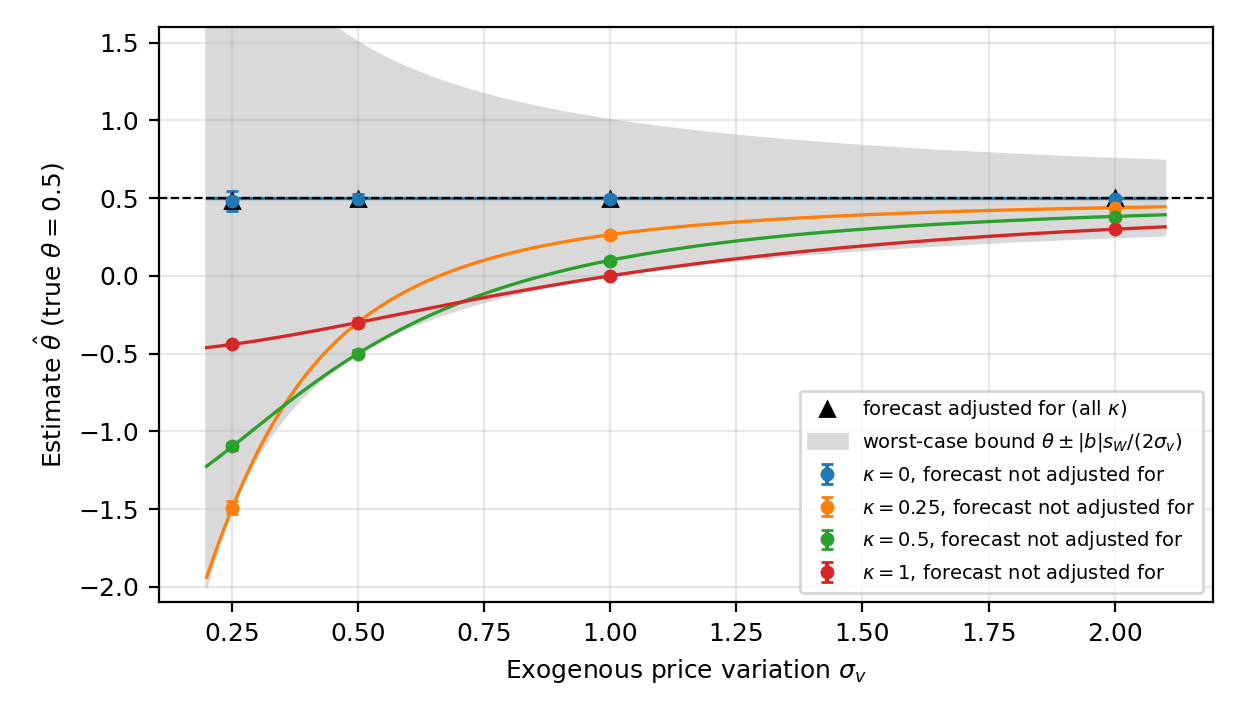
\includegraphics[width=0.8\linewidth]{figures/reactive.png}
\caption{Study 1. Mean estimate ($\pm$ one standard deviation across replications) against exogenous price variation, by the share $\kappa$ of unobserved difficulty the forecast sees. Lines are Proposition~\ref{prop:bias}; the band is the second bound of Corollary~\ref{cor:bounds}; triangles adjust for the forecast.}
\label{fig:reactive}
\end{figure}

\paragraph{Reactive pricing.} The estimates follow Proposition~\ref{prop:bias} closely (Figure~\ref{fig:reactive}): across the twelve biased cells the mean estimate is within \SoneMaxDev\ of the closed form, for example \SoneExTheta\ against \SoneExAnalytic\ at $\kappa = 1$, $\sigma_v = 0.5$, and \SoneBoundTheta\ at $\kappa = 0.25$, $\sigma_v = 0.25$, where the bound is attained. With $\kappa = 0$, price reacts as strongly to observable difficulty but the estimate is unbiased. At $\kappa = 1$, overlap is between \SoneKoneOvMin\ and \SoneKoneOvMax\ while the estimate ranges from \SoneKoneThetaMin\ to \SoneKoneThetaMax. Adjusting for the forecast recovers the effect (mean estimates \SoneLoggedThetaMin\ to \SoneLoggedThetaMax) and lowers overlap to the exogenous share, as low as \SoneLoggedOvMin. Across the unbiased cells, those with $\kappa = 0$ and those that adjust for the forecast, coverage is between \SoneUnbCovMin\ and \SoneUnbCovMax, slightly below nominal. The standard error is well calibrated (the median ratio of the mean standard error to the standard deviation of the estimates is \SoneSESDMedian); the shortfall comes from a small finite-sample bias of \SoneBiasSDMin\ to \SoneBiasSDMax\ standard deviations, the regularization bias of the penalized nuisance fits, whose errors in $h(X)$ enter the price and outcome residuals together. The ratio falls to \SoneLoggedSESDMin\ only in the forecast-adjusted cells with the least exogenous variation.

\begin{figure}[!htbp]
\centering
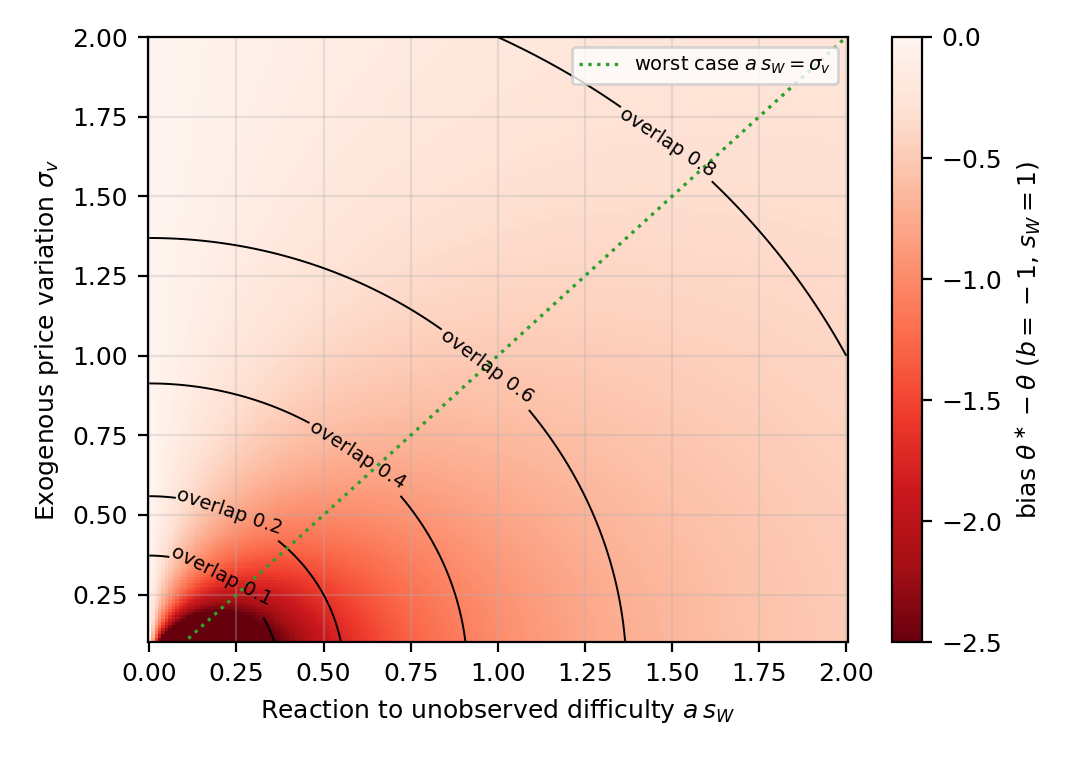
\includegraphics[width=0.66\linewidth]{figures/bias_map.png}
\caption{Proposition~\ref{prop:bias} for the reactive model ($b = -1$, $s_W = 1$). Shading is the bias; lines are overlap contours. Along any contour the bias ranges from zero, when the residual variation is exogenous, to large values, when it is confounded.}
\label{fig:map}
\end{figure}

Figure~\ref{fig:map} shows why overlap cannot track the bias. Overlap depends on the total residual variation $a^2 s_W^2 + \sigma_v^2$, so its contours are circles in the $(a s_W, \sigma_v)$ plane; the bias depends on the angle, and moves from zero to its maximum along each contour.

\begin{figure}[!htbp]
\centering
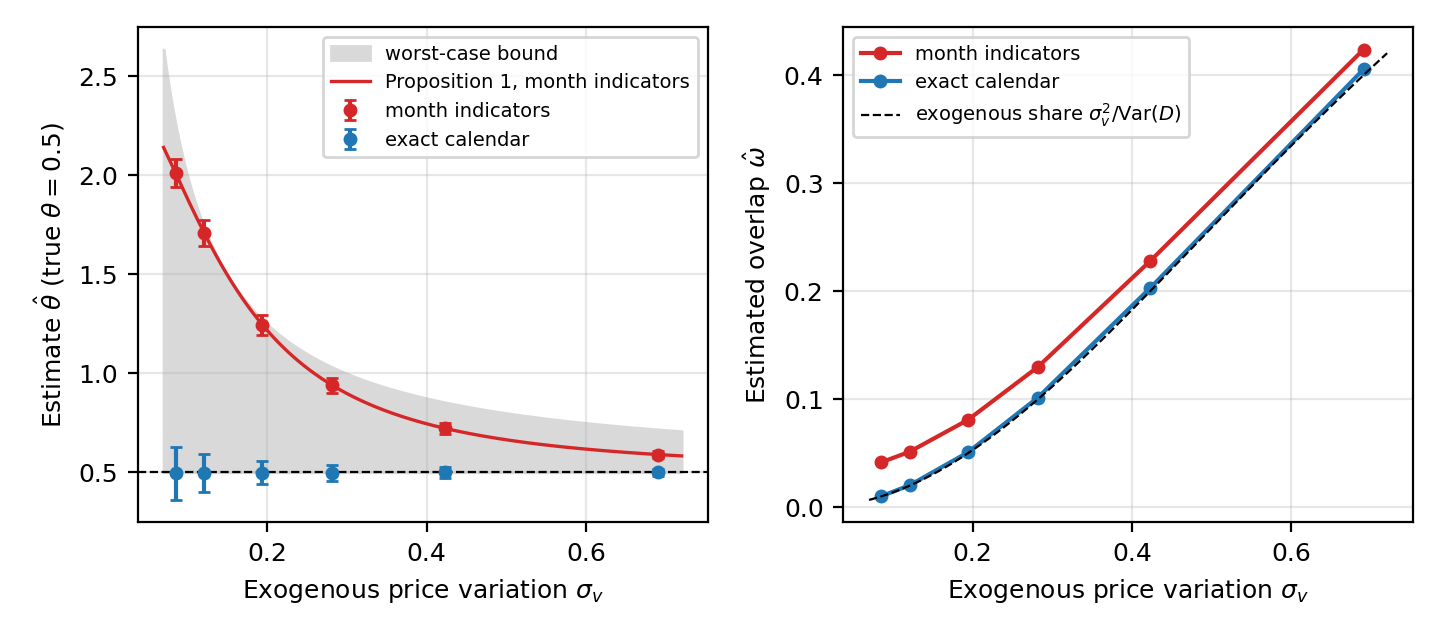
\includegraphics[width=\linewidth]{figures/coarse_calendar.png}
\caption{Study 2, spline learner. Left: mean estimate ($\pm$ one standard deviation) with exact calendar adjustment and with month indicators; the line is Proposition~\ref{prop:bias} and the band the second bound of Corollary~\ref{cor:bounds}. Right: estimated overlap; the dashed line is the exogenous share.}
\label{fig:coarse}
\end{figure}

\begin{figure}[!htbp]
\centering
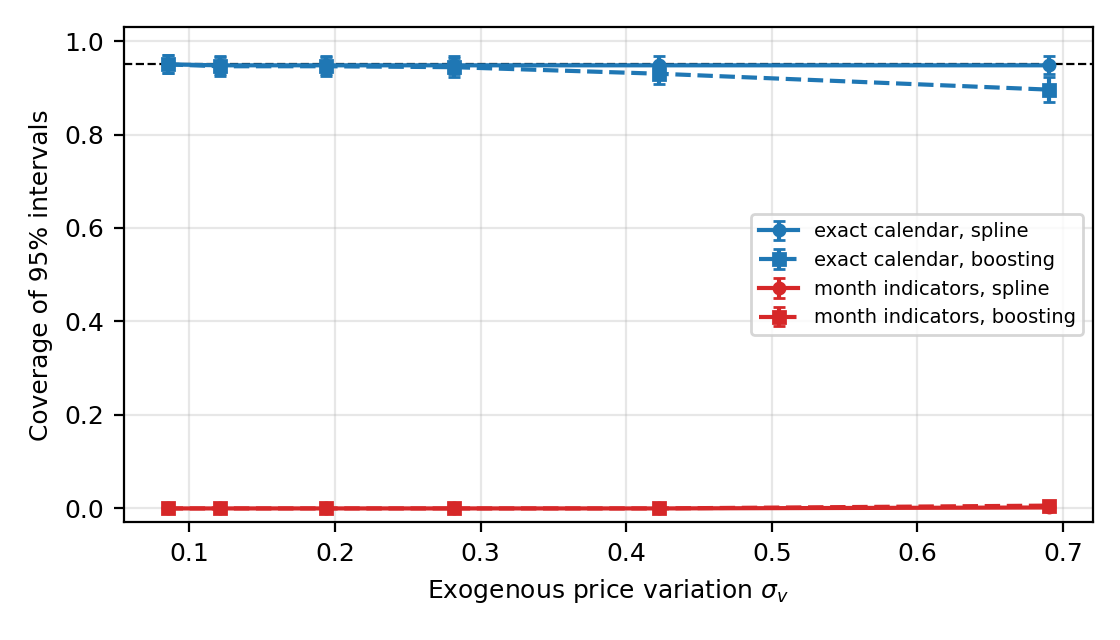
\includegraphics[width=0.66\linewidth]{figures/coverage.png}
\caption{Study 2. Coverage of 95\% intervals with 95\% Monte Carlo error bars, by calendar adjustment and learner.}
\label{fig:coverage}
\end{figure}

\paragraph{Approximate adjustment.} With exact calendar adjustment the estimate is unbiased at every level of overlap (largest absolute bias \StwoExactMaxAbsBias), and coverage is between \StwoExactCovMin\ and \StwoExactCovMax\ (Figures~\ref{fig:coarse} and~\ref{fig:coverage}). Weak overlap widens the interval, from a standard error of \StwoExactSEhigh\ at overlap 0.4 to \StwoExactSElow\ at 0.01, but does not invalidate it. With month indicators the estimates match Proposition~\ref{prop:bias} to within \StwoMonthMaxDev, the bias grows from \StwoMonthBiasLow\ at the largest exogenous variation to \StwoMonthBiasHigh\ at the smallest, where the estimate is \StwoMonthThetaHigh\ against a true effect of 0.5, and coverage is at most \StwoMonthCovMax. Overlap does not warn: month indicators raise it above the exogenous share, from \StwoOvExactLow\ to \StwoOvMonthLow\ at the smallest exogenous variation. With gradient boosting, the coarse-calendar estimate at the smallest exogenous variation is \StwoBoostMonthThetaHigh; with exact adjustment, boosting has a small downward bias (at most \StwoBoostExactMaxAbsBias) from its slower-converging nuisance fits, and coverage between \StwoBoostExactCovMin\ and \StwoBoostExactCovMax.

\begin{figure}[!htbp]
\centering
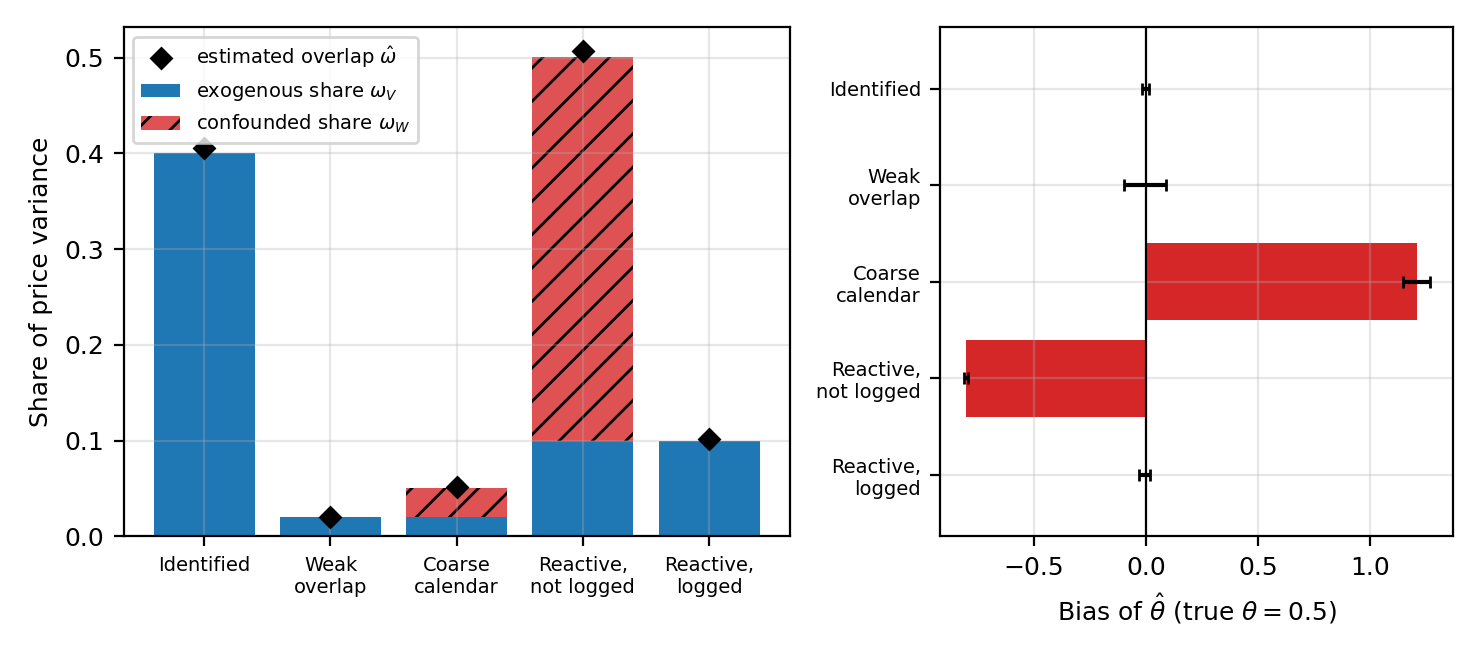
\includegraphics[width=\linewidth]{figures/overlap_decomposition.png}
\caption{Study 3. Left: population exogenous share $\omega_V$ and confounded share $\omega_W$ of price variance, with the mean estimated overlap. Right: mean bias ($\pm$ one standard deviation).}
\label{fig:decomp}
\end{figure}

\begin{table}[!htbp]
\caption{Study 3. Mean estimate, coverage, estimated overlap $\hat\omega$, and the population exogenous and confounded shares ($\theta = 0.5$).}
\label{tab:diagnostics}
\centering
\small
\begin{tabular}{lrrrrrr}
\toprule
Scenario & Bias & $\hat\theta$ & Coverage & $\hat\omega$ & $\omega_V$ & $\omega_W$ \\
\midrule
Identified & 0 & 0.499 & 94.6\% & 0.405 & 0.400 & 0.000 \\
Weak overlap & 0 & 0.497 & 94.6\% & 0.020 & 0.020 & 0.000 \\
Coarse calendar & 1.21 & 1.706 & 0.0\% & 0.051 & 0.020 & 0.031 \\
Reactive, forecast not logged & $-$0.80 & $-$0.301 & 0.0\% & 0.507 & 0.100 & 0.400 \\
Reactive, forecast logged & 0 & 0.494 & 93.8\% & 0.102 & 0.100 & 0.000 \\
\bottomrule
\end{tabular}

\end{table}

\paragraph{Overlap across scenarios.} Figure~\ref{fig:decomp} and Table~\ref{tab:diagnostics} show the decomposition at work. Estimated overlap matches $\omega_V + \omega_W$ in every scenario. It is highest, \SthreeReactOv, in the scenario where the estimate has the wrong sign, and it is higher with a coarse calendar (\SthreeCoarseOv) than with a correctly adjusted calendar and the same exogenous variation (\SthreeWeakOv). Confounded variation also makes a biased estimate look more precise. With the same exogenous share, the mean standard error is \SthreeSECoarse\ with the coarse calendar against \SthreeSEWeak\ with the exact one, and \SthreeSEUnlogged\ without the forecast against \SthreeSELogged\ with it: the scenarios with $\omega_W > 0$ report narrower intervals around the wrong value. Other routine checks behave as expected for checks of estimation rather than identification: the dispersion of the estimate across sample splits is between \SthreeDispMin\ and \SthreeDispMax\ standard errors in every scenario, the gap between the spline and boosting estimates is between \SthreeGapMin\ and \SthreeGapMax\ standard errors with no pattern by bias, and permutation placebos reject at \SthreePlacMin\ to \SthreePlacMax.

\paragraph{Bounds.} In the coarse-calendar scenario, $\mathrm{sd}(\tilde D) = \SthreeCoarseSD$ and the true $|b|\,s_W = \SthreeCoarseBS$, so the observed-quantity bound is $\SthreeCoarseBound$; with the exogenous fraction $\rho = \SthreeCoarseRho$, the exact expression in~\eqref{eq:bounds} reproduces the bias. The tipping point is $\tau = \SthreeCoarseTau$, slightly above $|b|\,s_W$: the unadjusted variation is large enough to multiply the estimate several times but not to explain all of it, which is correct, since the true effect is 0.5.

\begin{table}[!htbp]
\caption{Study 4. A difficulty function with an interaction and no confounding (population bias zero). The last column is Proposition~\ref{prop:bias} with $W = X_3 X_4$, the part of $h(X)$ an additive learner cannot represent.}
\label{tab:harder}
\centering
\small
\begin{tabular}{lrrrrrr}
\toprule
Learner & $\sigma_v$ & Bias & SD & Coverage & $\hat\omega$ & Proposition~\ref{prop:bias} \\
\midrule
Additive spline & 0.5 & $-$0.801 & 0.015 & 0.0\% & 0.567 & $-$0.800 \\
Additive spline & 1 & $-$0.503 & 0.014 & 0.0\% & 0.678 & $-$0.500 \\
Additive spline & 2 & $-$0.203 & 0.010 & 0.0\% & 0.844 & $-$0.200 \\
\addlinespace
Spline with $X_3 X_4$ & 0.5 & $-$0.008 & 0.033 & 93.6\% & 0.113 & 0 \\
Spline with $X_3 X_4$ & 1 & $-$0.005 & 0.016 & 93.2\% & 0.338 & 0 \\
Spline with $X_3 X_4$ & 2 & $-$0.003 & 0.008 & 92.2\% & 0.675 & 0 \\
\addlinespace
Random forest & 0.5 & $-$0.649 & 0.020 & 0.0\% & 0.370 & -- \\
\addlinespace
Boosting, defaults & 0.5 & $-$0.309 & 0.029 & 0.0\% & 0.178 & -- \\
Boosting, defaults & 1 & $-$0.119 & 0.017 & 0.0\% & 0.401 & -- \\
Boosting, defaults & 2 & $-$0.041 & 0.009 & 0.2\% & 0.727 & -- \\
\addlinespace
Boosting, tuned & 0.5 & $-$0.317 & 0.032 & 0.0\% & 0.179 & -- \\
Boosting, tuned & 1 & $-$0.128 & 0.017 & 0.0\% & 0.411 & -- \\
Boosting, tuned & 2 & $-$0.053 & 0.009 & 0.0\% & 0.741 & -- \\
\bottomrule
\end{tabular}

\end{table}

\paragraph{A harder nuisance function.} Table~\ref{tab:harder} shows what happens when the nuisance model, rather than the covariate set, falls short. Two learners serve as references. The additive spline cannot represent $X_3 X_4$, which is therefore left unadjusted exactly as in~\eqref{eq:structure}, with $W = X_3 X_4$, $a = 1$, and $b = -1$; its estimates match Proposition~\ref{prop:bias} to within \SfourSplineMaxDev. The same spline with the product $X_3 X_4$ added as a feature represents $h(X)$ exactly, and on the same data and folds its bias is at most \SfourIntMaxAbsBias\ in absolute value, with coverage of \SfourIntCovMin\ to \SfourIntCovMax, so the bias of the other learners comes from their nuisance fits and not from the cross-fitting or the estimator. The flexible learners fall in between. Boosting's bias ranges from \SfourBoostBiasLow\ at the largest exogenous variation to \SfourBoostBiasHigh\ at the smallest, tuning does not reduce it at this sample size (\SfourTunedBiasHigh), and a random forest is worse (\SfourRFBias). None reaches nominal coverage (at most \SfourCovMax), although their standard errors match the spread of the estimates (ratios \SfourSESDMin\ to \SfourSESDMax). The orthogonal score removes the first-order effect of nuisance error, but the product of the two nuisance errors remains and is divided by $\Var(\tilde D)$, so it grows as exogenous variation shrinks.

\begin{figure}[!htbp]
\centering
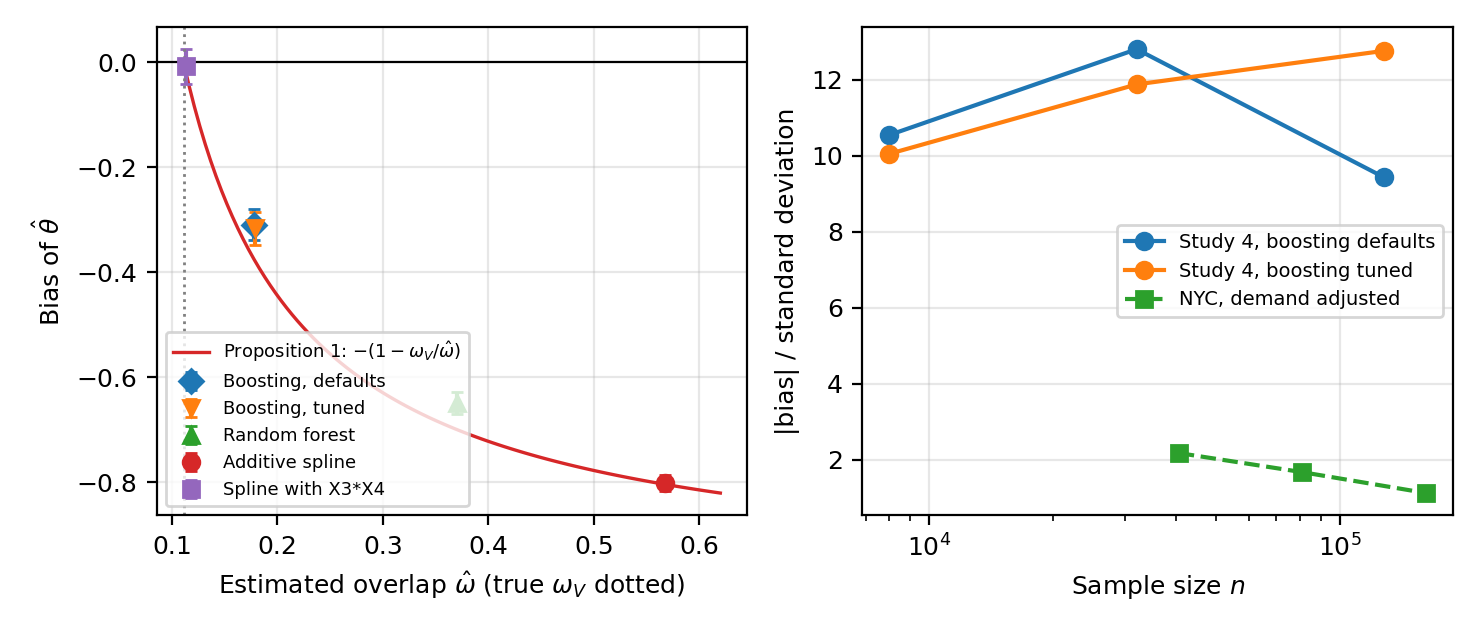
\includegraphics[width=\linewidth]{figures/nuisance_error.png}
\caption{Nuisance error as an unadjusted component. Left: Study 4 at $\sigma_v = 0.5$; bias against estimated overlap by learner ($\pm$ one standard deviation), with the curve Proposition~\ref{prop:bias} implies when the excess of $\hat\omega$ over the true exogenous share $\omega_V$ (dotted) is confounded variation. Right: $|$bias$|$ divided by the standard deviation of the estimate against sample size, for Study 4 at $\sigma_v = 0.5$ and for the demand-adjusted estimate in the semi-synthetic study (Section~\ref{sec:app}). The default learner's ratio falls at $n = 128{,}000$ only because its estimate becomes noisier there: above 10{,}000 observations it turns on early stopping with a random validation set, and its bias does not change.}
\label{fig:nuisance}
\end{figure}

Figure~\ref{fig:nuisance} (left) shows that nuisance error behaves like the unadjusted component of Section~\ref{sec:theory}. Whatever part of $h(X)$ a learner fails to capture stays in the price residual and inflates estimated overlap above the true exogenous share, and the bias tracks that inflation: the learners order by bias exactly as they order by overlap, and the two splines lie on the curve $-(1 - \omega_V / \hat\omega)$ that Proposition~\ref{prop:bias} implies when the excess overlap is confounded. Nuisance error, in other words, is one more source of $W$, and estimated overlap that exceeds what the design should allow is a symptom of it.

\paragraph{Sample size.} DML's guarantees require the product of the two nuisance errors to shrink faster than $n^{-1/2}$. We repeat the $\sigma_v = 0.5$ design at $n = 32{,}000$ and $128{,}000$ (Figure~\ref{fig:nuisance}, right), with \SfourDefRepsThirtyTwo\ replications at each size for the default learner and \SfourTunedRepsThirtyTwo\ and \SfourTunedRepsOneTwentyEight\ for the slower tuned learner. Boosting at default settings, which caps the number of trees, does not improve: its bias is \SfourDefBiasEight, \SfourDefBiasThirtyTwo, and \SfourDefBiasOneTwentyEight\ at the three sample sizes. The tuned learner, whose capacity grows with the data through early stopping, improves steadily: its bias falls from \SfourTunedBiasEight\ to \SfourTunedBiasThirtyTwo\ and \SfourTunedBiasOneTwentyEight, and its estimated overlap falls toward the true exogenous share, from \SfourTunedOvEight\ to \SfourTunedOvOneTwentyEight. Its standard error falls faster, however, halving with each fourfold increase in $n$ while the bias shrinks by less, so the bias grows from \SfourTunedBiasSDEight\ to \SfourTunedBiasSDOneTwentyEight\ standard deviations: for this function, at these sample sizes, the rate condition is not met. (Above 10{,}000 observations, the default learner also turns on early stopping with a random validation set, which makes its fits, and the estimate, more variable than its standard error indicates.)

\section{Semi-synthetic study: New York City rideshare pay}
\label{sec:app}

\paragraph{Data.} Delivery platforms do not publish pay and demand at a fine enough grain for this exercise, so we use rideshare, the closest public analogue: drivers are independent, pay is set by an algorithm subject to a regulated floor, and demand varies sharply by place and hour. We use the New York City high-volume for-hire vehicle trip records for March 2023~\citep{tlc2023}, which report driver pay, trip distance, and pickup zone and time for every trip. We aggregate trips to zone-hour cells, keep zones observed in at least 95\% of hours and cells with at least ten trips, and trim pay per mile at its 1st and 99th percentiles, leaving \AppN\ cells in \AppZones\ zones. The treatment is driver pay per mile (mean \$\AppPayMean, standard deviation \$\AppPaySD). Pay, demand (log trips), zone, and hour are the real data and keep their real joint distribution; only the outcome is simulated, so the true effect is known.

\paragraph{Design.} The outcome is $Y = \theta D + 0.3\,\bar q_z + s(\text{hour of week}) - q^{\ast} + \varepsilon$, with $\theta = 0.5$, $\bar q_z$ the zone's mean log demand, $s$ the standardized real hour-of-week profile of log demand, $q^{\ast}$ the demand surprise (log trips net of zone and hour-of-week effects, standard deviation \AppSurpriseSD), and $\varepsilon \sim N(0, 0.5^2)$. Pay per mile co-moves with the demand surprise (slope \$\AppSlope\ per mile per log unit, Figure~\ref{fig:appdata}), so demand acts as a confounder. The co-movement need not come from a pricing algorithm reacting to a forecast: driver pay in these records is subject to the Taxi and Limousine Commission's minimum pay standard, which has per-mile and per-minute components, so pay per mile rises mechanically when trips slow down, and congestion moves with demand. Because the outcome is simulated, the validity of the study does not depend on why pay moves. We estimate $\theta$ with gradient boosting (zone and calendar as categorical features), five folds, and \AppDraws\ outcome draws, under three adjustment sets: zone and hour of week, which omits demand; zone, hour of week, and demand, which adjusts for the confounder; and zone, day part (six four-hour blocks by weekday or weekend), and demand, which adjusts for the calendar coarsely. Standard errors are heteroskedasticity-robust rather than clustered by zone. Pay and demand are correlated within zones, but the simulated outcome noise is independent across cells, so the robust variance describes the sampling variation in this design; with real outcomes, which share zone-level shocks, zone-clustered errors would be needed. Because the nuisance fits are not additive here, we evaluate Proposition~\ref{prop:bias} with the estimator's own cross-fitted residuals: the predicted bias is the slope of the unadjusted demand surprise and seasonal component on the pay residual, times their outcome loadings.

\begin{figure}[!htbp]
\centering
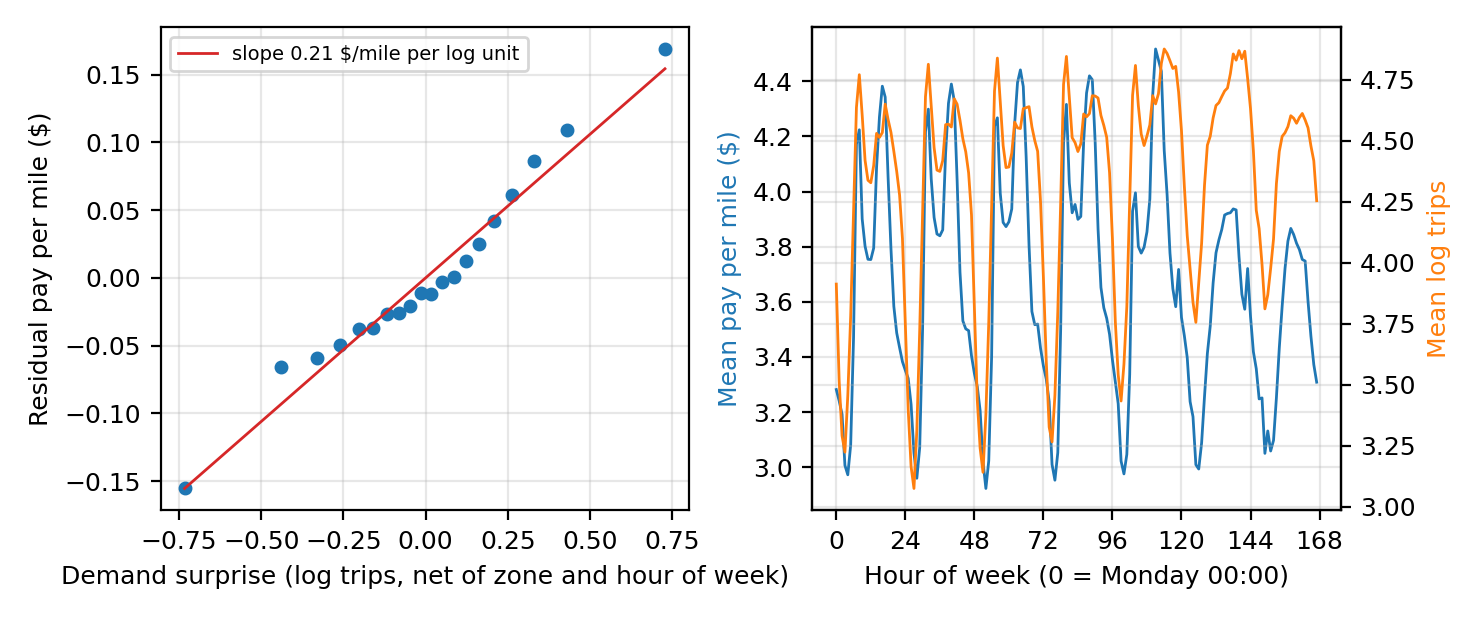
\includegraphics[width=\linewidth]{figures/application_data.png}
\caption{NYC rideshare data, March 2023. Left: residual pay per mile against the demand surprise, in 20 quantile bins. Right: mean pay per mile and mean log trips by hour of week.}
\label{fig:appdata}
\end{figure}

\begin{table}[!htbp]
\caption{Semi-synthetic study ($\theta = 0.5$, \AppDraws\ outcome draws). Predicted bias is Proposition~\ref{prop:bias} evaluated with the estimator's cross-fitted residuals; the tipping point is $|\hat\theta|\,\mathrm{sd}(\tilde D)$.}
\label{tab:app}
\centering
\small
\begin{tabular}{lrrrrrr}
\toprule
Adjustment set & $\hat\theta$ & Bias & Predicted bias & Coverage & $\hat\omega$ & Tipping point \\
\midrule
Zone, hour of week & 0.434 & $-$0.066 & $-$0.043 & 0\% & 0.155 & 0.107 \\
Zone, hour of week, demand & 0.494 & $-$0.006 & 0.001 & 83\% & 0.155 & 0.121 \\
Zone, day part, demand & 0.761 & 0.261 & 0.263 & 0\% & 0.214 & 0.219 \\
\bottomrule
\end{tabular}

\end{table}

\begin{figure}[!htbp]
\centering
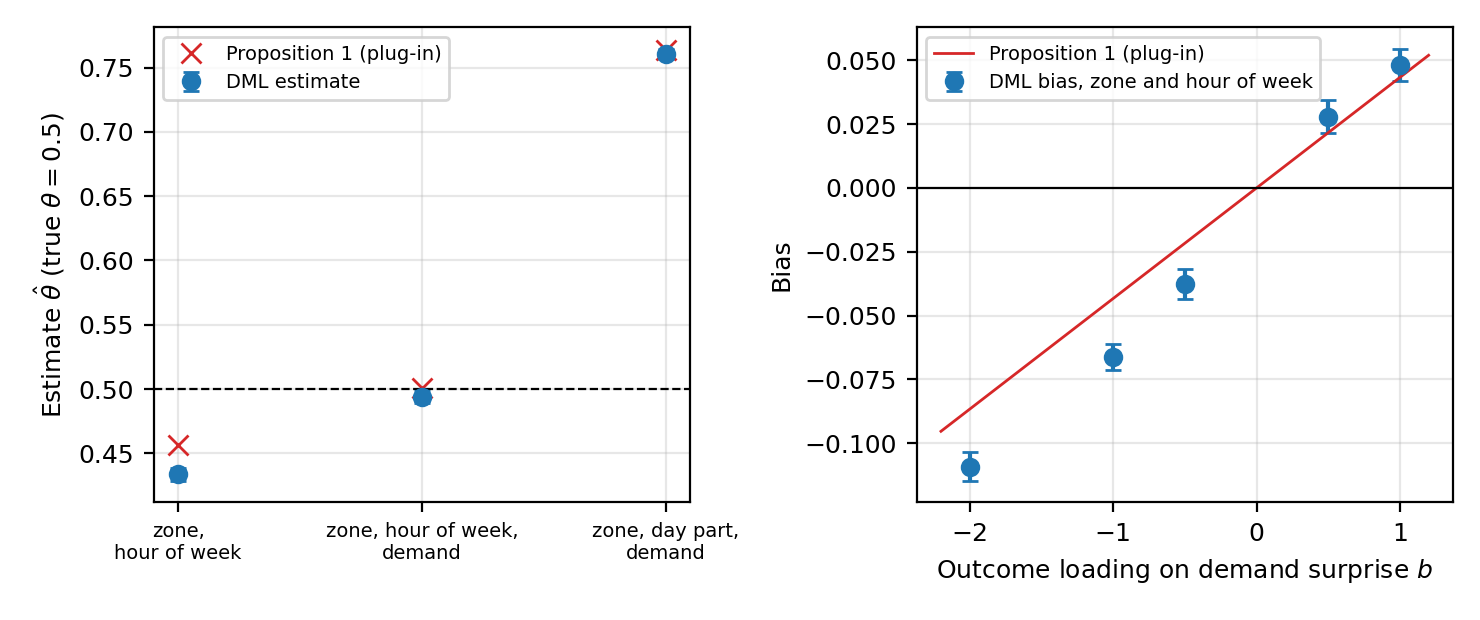
\includegraphics[width=\linewidth]{figures/application_estimates.png}
\caption{Semi-synthetic study. Left: estimates ($\pm$ one standard deviation across draws) and the plug-in prediction of Proposition~\ref{prop:bias}, by adjustment set. Right: bias against the outcome's loading on the demand surprise, without adjusting for demand.}
\label{fig:appest}
\end{figure}

\paragraph{Results.} Table~\ref{tab:app} and Figure~\ref{fig:appest} report the estimates. Omitting demand gives \AppATheta\ (bias \AppABias, predicted \AppAPred), and adjusting for it gives \AppBTheta\ (bias \AppBBias); overlap is unchanged at \AppBOv, because pay co-moves with the demand surprise only weakly once zone and hour of week are fixed. The coarse calendar is the larger problem in these data: with day parts in place of hours, the estimate is \AppCTheta\ (bias \AppCBias, predicted \AppCPred), while overlap rises to \AppCOv. The plug-in prediction captures the coarse-calendar bias almost exactly and about two thirds of the omitted-demand bias; the gap reflects the one difference between the two calculations, which is that the prediction uses a separate nuisance fit of the surprise while the estimator absorbs it through the outcome model. Because the standard errors are small here, a modest bias is many standard errors: coverage is \AppACov\ for both biased adjustment sets and \AppBCov\ with demand adjusted, over the \AppDraws\ draws of Table~\ref{tab:app}. The last figure is clearly below nominal, and we checked whether a better learner fixes it. On a separate set of \AppTuneDraws\ draws (Monte Carlo standard error of coverage about \AppTuneMCSE\ points), coverage is \AppTuneDefCov\ with the learner above and \AppTuneTunedCov\ with a tuned one (learning rate 0.05, up to 2{,}000 trees with 63 leaves, early stopping), and the bias is \AppTuneDefBias\ in both. The standard error is not the problem: it matches the spread of the estimates (ratio \AppTuneDefSESD). The bias is, at \AppTuneDefBiasSD\ standard deviations. It is the second-order remainder that the orthogonal score does not remove, the product of the errors in the two nuisance fits divided by $\Var(\tilde D)$. With \AppN\ cells the standard error is only \AppTuneDefSE, so a remainder that is negligible in absolute terms is a full standard deviation, and a tuned learner did not shrink it. It does shrink with the sample, faster than the standard error. On a third set of draws, \AppSubDraws\ for each sample size, re-estimating on random subsamples of \AppSubQuarterN\ and \AppSubHalfN\ cells gives biases of \AppSubQuarterBias\ and \AppSubHalfBias\ (\AppSubQuarterBiasSD\ and \AppSubHalfBiasSD\ standard deviations, coverage \AppSubQuarterCov\ and \AppSubHalfCov), against \AppSubFullBias\ (\AppSubFullBiasSD\ standard deviations, coverage \AppSubFullCov) on all cells (Figure~\ref{fig:nuisance}, right). The full-sample figures from the three sets of draws, a bias of \AppBBias, \AppTuneDefBias, and \AppSubFullBias\ and coverage of \AppBCov, \AppTuneDefCov, and \AppSubFullCov, differ only by Monte Carlo error. Intervals for estimates this precise should be read with that remainder in mind. The right panel of Figure~\ref{fig:appest} shows the bias scaling linearly with the outcome's sensitivity to the omitted demand, as Proposition~\ref{prop:bias} implies. The magnitudes are specific to this outcome model; the qualitative lesson, that the coarse adjustment raised overlap while producing the larger bias, does not depend on it.

\section{A delivery-style study calibrated to public data}
\label{sec:delivery}

The rideshare study keeps real covariates, but its pay moves through a regulated pay formula rather than a pricing rule that reacts to a forecast. This section shows that mechanism in a delivery setting, calibrated to public data on app-based restaurant delivery in New York City published by the Department of Consumer and Worker Protection~\citep{dcwp2026report, dcwp2026data}. Those data are citywide aggregates, too coarse to estimate a price effect from, but they pin down the setting: we take the week-to-week pattern of supply slack from the agency's weekly utilization series (the share of couriers' online time spent on deliveries), using its first 13 weeks, from the week of December 28, 2020 to the week of March 22, 2021, and the level of hourly pay, \$21.63 per hour excluding tips, from the second quarter of 2026. The two come from different periods, because the utilization series ends in June 2022; we use them to set the shape of week-to-week variation and the level of pay, not to reconstruct any particular period. The demand profile, with lunch and dinner peaks and busier weekend evenings, the dispersion of pay (standard deviation \$\DelPaySD), and the outcome are assumed.

\paragraph{Design.} A panel of \DelZones\ delivery zones by hour over \DelWeeks\ weeks (\DelN\ zone-hours). A zone-hour's shortfall of couriers depends on the zone, the hour of week, the week's supply slack, a demand shock that persists from one week to the next at the same zone and hour, and a real-time supply shock. The platform forecasts the shortfall from inputs it logs, the zone, the hour of week, the same hour's demand a week earlier, and the previous week's utilization, and, in one version, also from the real-time supply shock, which the analyst's data do not contain. Hourly pay reacts to the forecast plus exogenous noise, so the exogenous share of pay variance is $\omega_V = \DelExo$. The outcome is the share of orders filled, which rises by $\theta = 0.5$ percentage points per \$1 per hour of pay and falls with the true shortfall. We estimate $\theta$ with gradient boosting, treating zone, hour of week, and week as categorical, under three adjustment sets: the calendar and zone only; adding the forecast's logged inputs; and adding the logged forecast itself. Proposition~\ref{prop:bias} gives the bias of each in closed form, and we report \DelDraws\ draws of each design.

\begin{table}[!htbp]
\caption{Delivery-style study ($\theta = 0.5$, \DelDraws\ draws). ``Proposition~\ref{prop:bias}'' is $\theta$ plus the closed-form bias; $\omega_V$ is the exogenous share of pay variance.}
\label{tab:delivery}
\centering
\small
\begin{tabular}{llrrrrr}
\toprule
Forecast & Adjustment set & $\hat\theta$ & Proposition~\ref{prop:bias} & Coverage & $\hat\omega$ & $\omega_V$ \\
\midrule
Logged inputs only & Zone, hour of week, week & 0.243 & 0.225 & 0\% & 0.287 & 0.200 \\
 & + logged forecast inputs & 0.486 & 0.500 & 61\% & 0.205 & 0.200 \\
 & + logged forecast & 0.491 & 0.500 & 82\% & 0.204 & 0.200 \\
\addlinespace
Also real-time supply & Zone, hour of week, week & $-$0.449 & $-$0.454 & 0\% & 0.683 & 0.200 \\
 & + logged forecast inputs & $-$0.427 & $-$0.429 & 0\% & 0.646 & 0.200 \\
 & + logged forecast & 0.490 & 0.500 & 67\% & 0.204 & 0.200 \\
\bottomrule
\end{tabular}

\end{table}

\begin{figure}[!htbp]
\centering
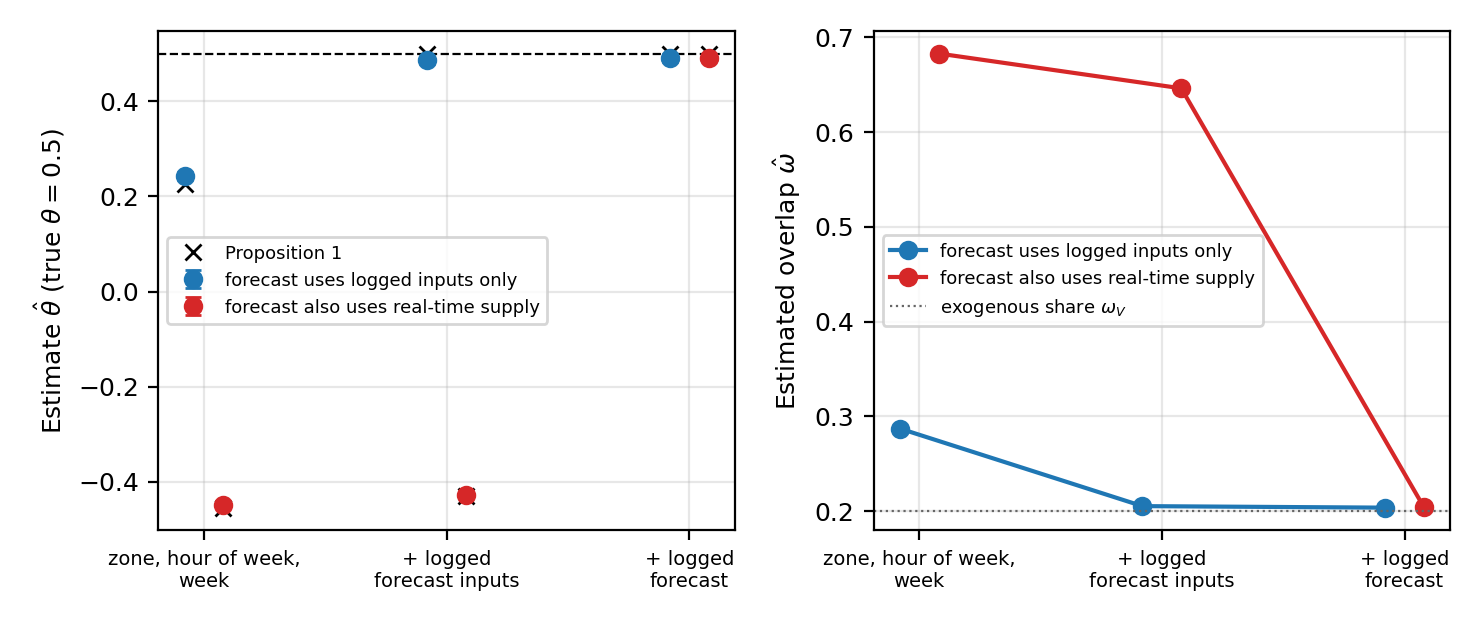
\includegraphics[width=\linewidth]{figures/delivery.png}
\caption{Delivery-style study. Left: estimates ($\pm$ one standard deviation across draws) and Proposition~\ref{prop:bias} (crosses), by adjustment set and by what the platform's forecast uses. Right: estimated overlap, with the exogenous share of pay variance dotted.}
\label{fig:delivery}
\end{figure}

\paragraph{Results.} Table~\ref{tab:delivery} and Figure~\ref{fig:delivery} report the estimates, which are within \DelMaxDev\ of Proposition~\ref{prop:bias} in every cell. When the forecast uses only logged inputs, adjusting for those inputs is enough: the estimate moves from \DelZeroATheta\ with the calendar alone to \DelZeroBTheta, and overlap falls from \DelZeroAOv\ to \DelZeroBOv, close to the exogenous share. When the forecast also uses real-time supply, adjusting for its logged inputs barely helps: the estimate is \DelOneBTheta\ against \DelOneATheta\ without them, with the wrong sign, and overlap stays at \DelOneBOv. Only adjusting for the logged forecast itself recovers the effect (\DelOneCTheta) and brings overlap down to the exogenous share (\DelOneCOv). The practical point refines Remark~\ref{rem:logging}: when a pricing rule uses information that is not stored with the transaction, logging the rule's inputs is not enough, and the forecast it acted on must be logged. As in the rideshare study, the unbiased estimates carry a small regularization bias (\DelUnbBiasMin\ to \DelUnbBiasMax) that is large relative to their standard errors (about \DelSE), so coverage there is \DelUnbCovMin\ to \DelUnbCovMax; this is the nuisance-error remainder of Section~\ref{sec:sims} (Study 4) and Section~\ref{sec:app}, which the orthogonal score does not remove and which is large here relative to standard errors computed from \DelN\ zone-hours.

\section{Evaluating the overlap-inflation diagnostic}
\label{sec:diag}

We evaluate the diagnostic on refinements whose truth we know (Table~\ref{tab:diagnostic}, Figure~\ref{fig:diagnostic}), with \DiagReps\ replications for each simulated case and 100 draws each for the rideshare and delivery pairs, which we re-estimate on shared folds so that the paired test can be computed. Five refinements remove confounded variation: month indicators to the exact calendar (Study 2), the additive spline to the spline with $X_3 X_4$ (Study 4), adding the forecast when it carries hidden information (Study 1, $\kappa = 1$), day parts to hours (rideshare), and logged forecast inputs to the logged forecast when the forecast uses real-time supply (delivery). Six start from a coarse residual with no confounded variation: the exact calendar to additional Fourier terms; adding a covariate that moves price but not the outcome; adding the forecast when it carries no hidden information, in Study 1 and in the delivery study; and, as negative controls for heterogeneous effects, the price-only covariate and the extra Fourier terms in a design where the effect varies, $\theta_i = 0.5 + \delta\,(\mathbf{1}\{X_2 > 0\} - 1/2)$, and the price-only covariate moves price only where $X_2 > 0$. With heterogeneous effects the partially linear estimand is a weighted average of $\theta_i$ with weights $\E[\tilde D^2 \mid X]$, so a refinement that removes price variation unevenly across $X$ changes the estimand without any confounding.

\begin{table}[!htbp]
\caption{The overlap-inflation diagnostic. ``Absorbed'' is the median share of the coarse residual price variance that the refinement removes. The pre-specified rule flags when that share exceeds 5\% and the conservative $|z|$ exceeds 2; the paired test flags when the paired $|z|$ exceeds 2. Columns $z$ are medians; ``Flagged'' columns are shares of replications.}
\label{tab:diagnostic}
\centering
\scriptsize
\setlength{\tabcolsep}{2.5pt}
\begin{tabular}{llrrrrrrr}
\toprule
 & & & & & \multicolumn{2}{c}{Pre-specified rule} & \multicolumn{2}{c}{Paired test} \\
\cmidrule(lr){6-7}\cmidrule(lr){8-9}
Refinement & Design & Level & Coarse bias & Absorbed & $z$ & Flagged & $z$ & Flagged \\
\midrule
\multicolumn{9}{l}{\emph{Coarse residual contains confounded variation}} \\
Month indicators $\to$ exact calendar & Study 2 & $\omega = 0.02$ & 1.205 & 60\% & 11.1 & 100.0\% & 16.7 & 100.0\% \\
Month indicators $\to$ exact calendar & Study 2 & $\omega = 0.1$ & 0.436 & 22\% & 8.2 & 100.0\% & 20.8 & 100.0\% \\
Month indicators $\to$ exact calendar & Study 2 & $\omega = 0.4$ & 0.088 & 4\% & 3.9 & 6.5\% & 15.2 & 100.0\% \\
Additive $\to$ interaction learner & Study 4 & $\sigma_v = 0.5$ & $-$0.802 & 80\% & $-$22.6 & 100.0\% & $-$27.2 & 100.0\% \\
Additive $\to$ interaction learner & Study 4 & $\sigma_v = 1$ & $-$0.504 & 50\% & $-$23.5 & 100.0\% & $-$35.0 & 100.0\% \\
Additive $\to$ interaction learner & Study 4 & $\sigma_v = 2$ & $-$0.203 & 20\% & $-$16.2 & 100.0\% & $-$27.8 & 100.0\% \\
$X \to X$ and forecast, $\kappa = 1$ & Study 1 & $\sigma_v = 0.5$ & $-$0.800 & 80\% & $-$31.8 & 100.0\% & $-$38.5 & 100.0\% \\
$X \to X$ and forecast, $\kappa = 1$ & Study 1 & $\sigma_v = 1$ & $-$0.502 & 50\% & $-$33.6 & 100.0\% & $-$51.4 & 100.0\% \\
$X \to X$ and forecast, $\kappa = 1$ & Study 1 & $\sigma_v = 2$ & $-$0.202 & 20\% & $-$22.7 & 100.0\% & $-$39.7 & 100.0\% \\
Day part $\to$ hour of week & Rideshare & -- & 0.261 & 28\% & 34.7 & 100.0\% & 58.3 & 100.0\% \\
Forecast inputs $\to$ forecast, real-time supply & Delivery & -- & $-$0.927 & 68\% & $-$125.1 & 100.0\% & $-$168.2 & 100.0\% \\
\addlinespace
\multicolumn{9}{l}{\emph{It does not}} \\
Exact calendar $\to$ more Fourier terms & Study 2 & $\omega = 0.02$ & $-$0.012 & 0\% & 0.0 & 0.0\% & 0.1 & 2.0\% \\
Exact calendar $\to$ more Fourier terms & Study 2 & $\omega = 0.1$ & $-$0.005 & 0\% & 0.0 & 0.0\% & 0.1 & 1.5\% \\
Exact calendar $\to$ more Fourier terms & Study 2 & $\omega = 0.4$ & $-$0.002 & 0\% & 0.0 & 0.0\% & 0.2 & 2.5\% \\
Without $\to$ with a price-only covariate & Study 2 & $\omega = 0.02$ & 0.000 & 86\% & 0.1 & 3.5\% & 0.2 & 6.5\% \\
Without $\to$ with a price-only covariate & Study 2 & $\omega = 0.1$ & $-$0.001 & 53\% & 0.1 & 0.5\% & 0.1 & 5.5\% \\
Without $\to$ with a price-only covariate & Study 2 & $\omega = 0.4$ & $-$0.001 & 15\% & 0.0 & 0.0\% & 0.1 & 6.5\% \\
$X \to X$ and forecast, $\kappa = 0$ & Study 1 & $\sigma_v = 0.5$ & $-$0.006 & 0\% & 0.0 & 0.0\% & 0.3 & 6.0\% \\
$X \to X$ and forecast, $\kappa = 0$ & Study 1 & $\sigma_v = 1$ & $-$0.003 & 0\% & 0.0 & 0.0\% & 0.9 & 13.0\% \\
$X \to X$ and forecast, $\kappa = 0$ & Study 1 & $\sigma_v = 2$ & $-$0.003 & 0\% & 0.1 & 0.0\% & 1.6 & 33.0\% \\
Forecast inputs $\to$ forecast, logged inputs only & Delivery & -- & $-$0.014 & 1\% & $-$0.4 & 0.0\% & $-$3.3 & 90.0\% \\
Without $\to$ with a price-only covariate & Heterogeneous & $\delta = 0$ & $-$0.001 & 39\% & 0.1 & 0.0\% & 0.2 & 6.0\% \\
Without $\to$ with a price-only covariate & Heterogeneous & $\delta = 0.1$ & 0.039 & 39\% & 0.4 & 0.0\% & 0.7 & 9.5\% \\
Without $\to$ with a price-only covariate & Heterogeneous & $\delta = 0.3$ & 0.119 & 39\% & 0.8 & 0.0\% & 1.6 & 30.5\% \\
Exact calendar $\to$ more Fourier terms & Heterogeneous & $\delta = 0$ & $-$0.004 & 0\% & 0.0 & 0.0\% & 0.0 & 3.0\% \\
Exact calendar $\to$ more Fourier terms & Heterogeneous & $\delta = 0.1$ & 0.030 & 0\% & 0.0 & 0.0\% & $-$0.1 & 2.5\% \\
Exact calendar $\to$ more Fourier terms & Heterogeneous & $\delta = 0.3$ & 0.097 & 0\% & 0.0 & 0.0\% & 0.0 & 3.5\% \\
\bottomrule
\end{tabular}

\end{table}

\begin{figure}[!htbp]
\centering
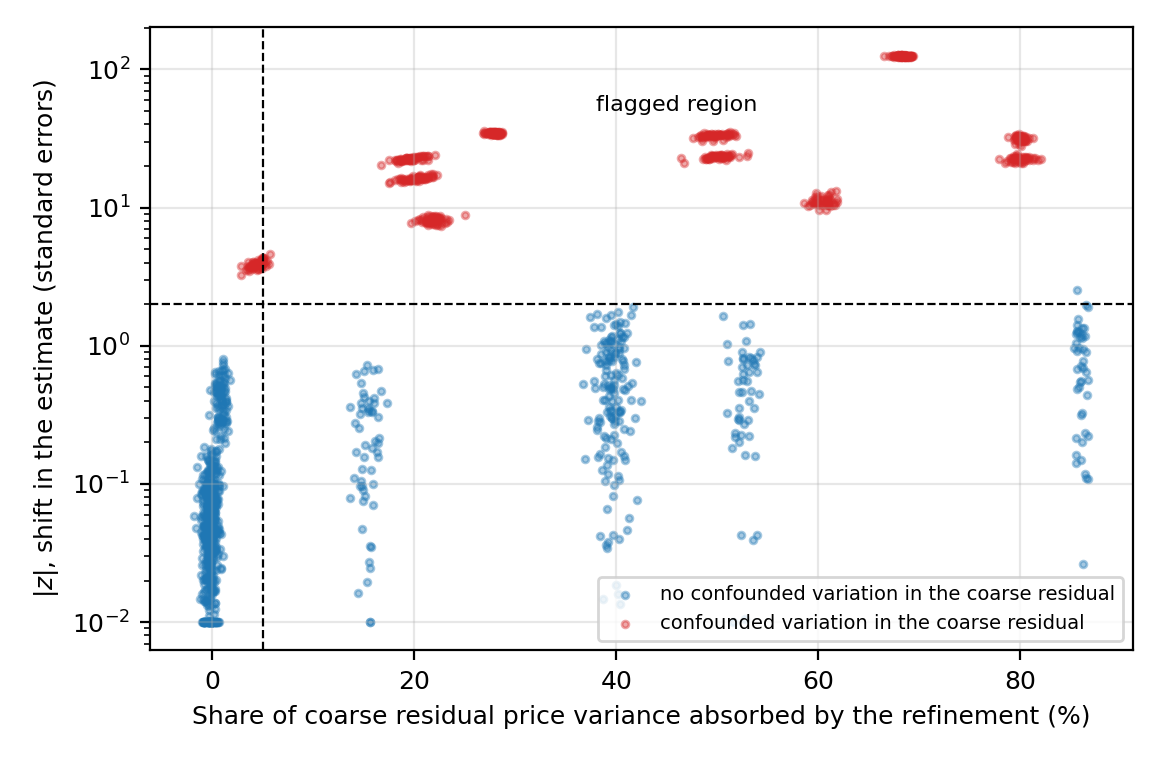
\includegraphics[width=0.72\linewidth]{figures/diagnostic.png}
\caption{The pre-specified rule. Each point is one replication of one refinement, plotted by the share of variance absorbed and the conservative shift; dashed lines are the flagging thresholds.}
\label{fig:diagnostic}
\end{figure}

\paragraph{The pre-specified rule.} The rule flags every replication in every case with confounded variation but one, and at most \DiagPreFPMax\ of replications in any case without, including all the heterogeneous-effect controls (at most \DiagHetPreMax). The most instructive negative case is the price-only covariate: adding it absorbs \DiagPriceOnlyAbsorbed\ of the residual price variance at the smallest exogenous variation, which a rule based on overlap alone would read as alarming, but the estimate does not move (median $|z| = \DiagPriceOnlyZ$), and the flag rate is \DiagPriceOnlyFlag. The rule misses the mildest case, the month-to-date refinement at the largest exogenous variation: the refinement absorbs only \DiagMissAbsorbed\ of the variance and removes a bias of \DiagMissBias, and although the conservative shift is large (median $|z| = \DiagMissZ$), the absorption condition holds in only \DiagMissFive\ of replications. A 2\% threshold would catch this case, but it would be tuned on these designs, so we report the rule as fixed in advance.

\paragraph{The paired test.} The paired test catches the mild case (median $|z| = \DiagMissZp$) and flags every replication of every confounded case, but it is not a test of confounding alone. It flags \DiagPairedRedundMin\ to \DiagPairedRedundMax\ of replications when a redundant forecast is added in Study 1 and \DiagPairedDelivery\ in the delivery study, where the two estimates differ by only \DiagDeliveryGap: adding an input that absorbs no price variation still changes the learner's fit slightly, and the difference between two nearly identical fits has a very small standard error, so a negligible shift becomes significant. It also responds to reweighting. In the heterogeneous design with $\delta = \DiagHetDelta$, adding the price-only covariate moves the estimand from \DiagHetCoarse\ to \DiagHetFine\ without any confounding, and the paired test flags \DiagHetPairedMax\ of replications, against \DiagHetPairedNull\ when the effect is homogeneous; the extra Fourier terms, which remove no price variation, are flagged at most \DiagHetFinerMax\ of the time. The paired test therefore answers a different question, whether the estimate changed by more than sampling noise, and its flags should be read as evidence of confounding only when effects are plausibly homogeneous and the refinement absorbs a material share of the price variation. We recommend the pre-specified rule, and the paired test as a more sensitive screen.

\section{Benchmarking the tipping point}
\label{sec:benchmark}

We compute the benchmarks of~\eqref{eq:benchmark} for the identified scenario of Study 3 (\BenchReps\ replications), the demand-adjusted rideshare estimate, and the forecast-adjusted delivery estimate (\BenchDraws\ draws each), estimating $g$ and $m$ with the same learners and folds as the effect, and we compare each benchmark with what actually happens when the group is dropped (Table~\ref{tab:benchmark}).

\begin{table}[!htbp]
\caption{Benchmarking the tipping point. $k_G$ and $t_G$ are a group's outcome-side and price-side strength beyond the other controls; $\tau / k_G$ is the one-sided worst case and $c^\ast_G$ the two-sided multiple~\eqref{eq:benchmark}; the last column is the change in the estimate, relative to the estimate, when the group is dropped. Means over replications, except medians for $c^\ast_G$ and the shift.}
\label{tab:benchmark}
\centering
\small
\begin{tabular}{llrrrrr}
\toprule
Study & Group $G$ & $k_G$ & $t_G$ & $\tau / k_G$ & $c^\ast_G$ & Shift if dropped \\
\midrule
Study 3 ($\tau = 0.350$) & calendar & 1.589 & 0.792 & 0.22 & 0.44 & +225\% \\
 & $X_1$ (price only) & 0.084 & 0.297 & 4.22 & 3.13 & 0\% \\
 & $X_2$ (outcome only) & 0.713 & 0.048 & 0.49 & 2.67 & 0\% \\
 & $X_3$ (outcome only) & 0.711 & 0.047 & 0.49 & 2.68 & 0\% \\
\addlinespace
Rideshare ($\tau = 0.121$) & zone & 0.332 & 0.316 & 0.36 & 0.53 & 0\% \\
 & hour of week & 0.612 & 0.300 & 0.20 & 0.40 & +98\% \\
 & demand & 0.151 & 0.052 & 0.80 & 1.93 & $-$12\% \\
\addlinespace
Delivery ($\tau = 0.497$) & zone & 0.231 & 0.106 & 2.15 & 4.53 & 0\% \\
 & hour of week & 0.271 & 0.125 & 1.83 & 3.86 & +1\% \\
 & week & 1.065 & 0.102 & 0.47 & 2.16 & +1\% \\
 & lagged demand & 0.226 & 0.102 & 2.19 & 4.67 & 0\% \\
 & forecast & 1.956 & 1.479 & 0.25 & 0.42 & $-$186\% \\
\bottomrule
\end{tabular}

\end{table}

The two-sided multiple separates the groups that matter from those that do not. It is below one for all three groups whose omission moves the estimate by more than its own size: the calendar in Study 3 ($c^\ast_G = \BenchCalC$; dropping it moves the estimate by \BenchCalShift), hour of week in the rideshare study (\BenchHowC; \BenchHowShift), and the logged forecast in the delivery study (\BenchFcC; \BenchFcShift). All other groups but one have $c^\ast_G$ of at least \BenchSafeCMin, and dropping any of them moves the estimate by at most \BenchSafeShiftMax. The remaining group falls below one without mattering, an error in the safe direction: zone in the rideshare study has $c^\ast_G = \BenchZoneC$, but dropping it moves the estimate by only \BenchZoneShift, because the multiple assumes a single component whose price and outcome parts are aligned, and zone's are not. The one-sided ratio is a poor guide: covariates that affect only the outcome have $\tau / k_G$ of about \BenchOutOnlyRatio, which suggests fragility, but $c^\ast_G$ of about \BenchOutOnlyC, and dropping them changes nothing. We therefore recommend reporting $c^\ast_G$ for the main groups of controls alongside $\tau$.

\section{Verifying the implementation}
\label{sec:doubleml}

To verify our implementation of the estimator, we re-estimate the key designs with the DoubleML package~\citep{bach2022} (version \DmlVersion), using its partially linear estimator with the partialling-out score, five folds, and the same learners: Study 1 with $\sigma_v = 0.5$ ($\kappa = 1$ with and without the forecast, and $\kappa = 0$, 200 replications each), Study 4 with $\sigma_v = 0.5$ (additive spline, spline with $X_3 X_4$, and boosting, 200 replications each), and the three adjustment sets of the semi-synthetic study (50 draws each). With the same fold assignment, the two implementations agree to machine precision in all \DmlRuns\ runs: the largest difference is \DmlMaxDiff\ in the estimates and \DmlMaxSEDiff\ in the standard errors. This verifies our implementation of the estimator and its variance: the biases in Study 4, including the undercoverage of boosting without confounding, are properties of DML with these learners, not of an error in our code. It does not, and is not meant to, validate the choice of learners, which uses the same learner objects in both implementations.

\section{Practical guidance}
\label{sec:practice}

\begin{enumerate}
\item \textbf{Log and adjust for the pricing rule's inputs.} The forecast, the state variables, and any manual adjustments are the most valuable covariates in an observational price study. Adjusting for them removes the reactive component without modeling the rule (Remark~\ref{rem:logging}).
\item \textbf{Read overlap as exogenous variation only after that adjustment.} Without the rule's inputs, overlap mixes exogenous and confounded variation and can be high when the estimate is badly biased.
\item \textbf{Adjust for strong confounders at full resolution.} When exogenous variation is scarce, a confounder that drives most of the price variation must be adjusted for almost exactly.
\item \textbf{Check for overlap inflation.} Re-estimate under a finer adjustment, such as a finer calendar, a more flexible learner, or an additional logged input. Flag the coarse estimate when the refinement absorbs more than 5\% of the coarse residual price variance and the estimate shifts by more than two standard errors, with $z$ computed from the sum of the two variances. Under a constant effect, a flag means the coarse residual contained confounded variation and the coarse estimate should not be reported; if overlap falls and the estimate does not move, the refinement only removed exogenous variation. The paired test of Section~\ref{sec:diagtheory} is more sensitive, but it also responds to small changes in the learner's fit and to reweighting under heterogeneous effects, so its flags call for a closer look rather than a verdict.
\item \textbf{Report a tipping point and benchmark it.} $\tau = |\hat\theta|\,\mathrm{sd}(\tilde D)$ is the smallest outcome-scale effect of an unadjusted component that could explain the estimate away; the multiple $c^\ast_G$ in~\eqref{eq:benchmark} says how that compares with the main groups of observed controls.
\item \textbf{Treat nuisance error as a source of bias when exogenous variation is scarce.} Compare learners, including ones that can represent interactions, and read very narrow intervals cautiously: the remainder the orthogonal score leaves behind is divided by $\Var(\tilde D)$, so it can be many standard errors, and it shrinks with the sample size only if the learner's own error does.
\item \textbf{Plan an experiment when the exogenous share is small.} A randomized price perturbation supplies exogenous variation of known size, which identifies the effect directly and makes the second bound of Corollary~\ref{cor:bounds} usable.
\end{enumerate}

\section{Limitations and conclusion}
\label{sec:limits}

The structure~\eqref{eq:structure} is linear in the unadjusted component and assumes a constant effect. With heterogeneous effects or nonlinear dependence on $W$, the closed form is a first-order approximation; the general bounds of \citet{chernozhukov2022} continue to apply. The simulations use additive designs and a correctly specified learner to separate identification from estimation error. With harder nuisance functions, regularization bias adds to the bias studied here; Study 4 shows it can dominate when exogenous variation is scarce: boosting reduces it relative to an additive learner, tuning did not reduce it further at $n = 8{,}000$, and with a tuned learner it shrinks as $n$ grows but more slowly than the standard error, so it grows relative to the standard error. The semi-synthetic study uses one month of one city's rideshare data, not delivery data, and a simulated outcome, so its magnitudes illustrate rather than estimate the bias in practice, and how closely they carry over to delivery platforms is untested. The delivery-style study is calibrated to citywide aggregates, the weekly utilization series and the level of pay, and its demand profile, pay dispersion, and outcome are assumed, so it demonstrates the mechanism in a delivery setting rather than measuring it. Under heterogeneous effects, a refinement that removes price variation unevenly changes the weights of the partially linear estimand, so the estimate can move without confounding; the pre-specified rule did not flag this in our negative controls, but the more sensitive paired test did, and neither can by itself tell confounding from reweighting. The overlap-inflation diagnostic can only find confounded variation that some available refinement absorbs: a component that no finer calendar, learner, or logged input captures leaves overlap and the estimate unchanged, and only the tipping point and its benchmarks speak to it.

Overlap is usually read as a measure of how well an effect is identified. For a continuous treatment set by an algorithm, it measures the sum of two things with opposite consequences. Separating them fully requires information the data alone do not contain, and on algorithmically priced platforms that information, the forecast the pricing rule acted on, can usually be recorded. Where it is not, comparing a coarse and a finer adjustment, and benchmarking the tipping point against what is observed, show how much of the reported overlap can be trusted.

\begin{thebibliography}{99}

\bibitem[Altonji et~al.(2005)]{altonji2005}
Altonji, J.~G., Elder, T.~E., and Taber, C.~R. (2005).
Selection on observed and unobserved variables: Assessing the effectiveness of Catholic schools.
\emph{Journal of Political Economy}, 113(1):151--184.

\bibitem[Bach et~al.(2022)]{bach2022}
Bach, P., Chernozhukov, V., Kurz, M.~S., and Spindler, M. (2022).
DoubleML: An object-oriented implementation of double machine learning in Python.
\emph{Journal of Machine Learning Research}, 23(53):1--6.

\bibitem[Berry(1994)]{berry1994}
Berry, S.~T. (1994).
Estimating discrete-choice models of product differentiation.
\emph{RAND Journal of Economics}, 25(2):242--262.

\bibitem[Berry et~al.(1995)]{blp1995}
Berry, S., Levinsohn, J., and Pakes, A. (1995).
Automobile prices in market equilibrium.
\emph{Econometrica}, 63(4):841--890.

\bibitem[Bojinov et~al.(2023)]{bojinov2023}
Bojinov, I., Simchi-Levi, D., and Zhao, J. (2023).
Design and analysis of switchback experiments.
\emph{Management Science}, 69(7):3759--3777.

\bibitem[Bottou et~al.(2013)]{bottou2013}
Bottou, L., Peters, J., Qui\~nonero-Candela, J., Charles, D.~X., Chickering, D.~M., Portugaly, E., Ray, D., Simard, P., and Snelson, E. (2013).
Counterfactual reasoning and learning systems: The example of computational advertising.
\emph{Journal of Machine Learning Research}, 14:3207--3260.

\bibitem[Chen and Sheldon(2016)]{chen2016}
Chen, M.~K. and Sheldon, M. (2016).
Dynamic pricing in a labor market: Surge pricing and flexible work on the Uber platform.
In \emph{Proceedings of the 2016 ACM Conference on Economics and Computation}, p.~455.

\bibitem[Chernozhukov et~al.(2018)]{chernozhukov2018}
Chernozhukov, V., Chetverikov, D., Demirer, M., Duflo, E., Hansen, C., Newey, W., and Robins, J. (2018).
Double/debiased machine learning for treatment and structural parameters.
\emph{The Econometrics Journal}, 21(1):C1--C68.

\bibitem[Chernozhukov et~al.(2022)]{chernozhukov2022}
Chernozhukov, V., Cinelli, C., Newey, W., Sharma, A., and Syrgkanis, V. (2022).
Long story short: Omitted variable bias in causal machine learning.
NBER Working Paper 30302.

\bibitem[Cinelli and Hazlett(2020)]{cinelli2020}
Cinelli, C. and Hazlett, C. (2020).
Making sense of sensitivity: Extending omitted variable bias.
\emph{Journal of the Royal Statistical Society: Series B}, 82(1):39--67.

\bibitem[Cohen et~al.(2016)]{cohen2016}
Cohen, P., Hahn, R., Hall, J., Levitt, S., and Metcalfe, R. (2016).
Using big data to estimate consumer surplus: The case of Uber.
NBER Working Paper 22627.

\bibitem[Crump et~al.(2009)]{crump2009}
Crump, R.~K., Hotz, V.~J., Imbens, G.~W., and Mitnik, O.~A. (2009).
Dealing with limited overlap in estimation of average treatment effects.
\emph{Biometrika}, 96(1):187--199.

\bibitem[D'Amour et~al.(2021)]{damour2021}
D'Amour, A., Ding, P., Feller, A., Lei, L., and Sekhon, J. (2021).
Overlap in observational studies with high-dimensional covariates.
\emph{Journal of Econometrics}, 221(2):644--654.

\bibitem[Department of Consumer and Worker Protection(2026a)]{dcwp2026report}
New York City Department of Consumer and Worker Protection (2026a).
NYC delivery workers: An update on the minimum pay rate. Report submitted to the New York City Council, October 2026.
\url{https://www.nyc.gov/assets/dca/downloads/pdf/media/NYC-Delivery-Workers-MPR-Update-October-2026.pdf}.

\bibitem[Department of Consumer and Worker Protection(2026b)]{dcwp2026data}
New York City Department of Consumer and Worker Protection (2026b).
Restaurant and grocery delivery app aggregated tables, and weekly utilization data for delivery apps. Accessed November 4, 2026.
\url{https://www.nyc.gov/site/dca/workers/Delivery-Worker-Public-Hearing-Minimum-Pay-Rate.page}.

\bibitem[Dud\'ik et~al.(2011)]{dudik2011}
Dud\'ik, M., Langford, J., and Li, L. (2011).
Doubly robust policy evaluation and learning.
In \emph{Proceedings of the 28th International Conference on Machine Learning}.

\bibitem[Hirano and Imbens(2004)]{hirano2004}
Hirano, K. and Imbens, G.~W. (2004).
The propensity score with continuous treatments.
In Gelman, A. and Meng, X.-L., editors, \emph{Applied Bayesian Modeling and Causal Inference from Incomplete-Data Perspectives}, pp.~73--84. Wiley.

\bibitem[Imbens(2003)]{imbens2003}
Imbens, G.~W. (2003).
Sensitivity to exogeneity assumptions in program evaluation.
\emph{American Economic Review}, 93(2):126--132.

\bibitem[Imbens and Rubin(2015)]{imbens2015}
Imbens, G.~W. and Rubin, D.~B. (2015).
\emph{Causal Inference for Statistics, Social, and Biomedical Sciences: An Introduction}.
Cambridge University Press.

\bibitem[Narita and Yata(2021)]{narita2021}
Narita, Y. and Yata, K. (2021).
Algorithm as experiment: Machine learning, market design, and policy eligibility rules.
arXiv:2104.12909 (first version titled ``Algorithm is experiment'').

\bibitem[New York City Taxi and Limousine Commission(2023)]{tlc2023}
New York City Taxi and Limousine Commission (2023).
TLC trip record data: High volume for-hire vehicle trip records, March 2023.
\url{https://www.nyc.gov/site/tlc/about/tlc-trip-record-data.page}.

\bibitem[Oster(2019)]{oster2019}
Oster, E. (2019).
Unobservable selection and coefficient stability: Theory and evidence.
\emph{Journal of Business \& Economic Statistics}, 37(2):187--204.

\bibitem[Robinson(1988)]{robinson1988}
Robinson, P.~M. (1988).
Root-N-consistent semiparametric regression.
\emph{Econometrica}, 56(4):931--954.

\bibitem[Rosenbaum(2002)]{rosenbaum2002}
Rosenbaum, P.~R. (2002).
\emph{Observational Studies}, 2nd ed.
Springer.

\bibitem[Rosenbaum and Rubin(1983)]{rosenbaum1983}
Rosenbaum, P.~R. and Rubin, D.~B. (1983).
The central role of the propensity score in observational studies for causal effects.
\emph{Biometrika}, 70(1):41--55.

\bibitem[Veitch and Zaveri(2020)]{veitch2020}
Veitch, V. and Zaveri, A. (2020).
Sense and sensitivity analysis: Simple post-hoc analysis of bias due to unobserved confounding.
In \emph{Advances in Neural Information Processing Systems}, 33.

\end{thebibliography}

\appendix

\section{Implementation}

All code is in Python with scikit-learn. The code, the stored simulation output, and the scripts that produce every number, table and figure in the paper are available at \url{https://github.com/vikranthreddymoola/overlap-is-not-identification} and archived on Zenodo, \href{https://doi.org/10.5281/zenodo.24000911}{doi:10.5281/zenodo.24000911}. The spline learner is a cubic B-spline basis with twelve knots per covariate followed by ridge regression with the penalty chosen by cross-validation from $10^{-3}$ to $10^{3}$. The boosting learner is scikit-learn's histogram-based gradient boosting regressor, with default settings in the simulations and 300 iterations with zone and calendar treated as categorical in the semi-synthetic study. Folds are drawn at random, with a new split for each repetition. The estimate in each split is $\sum_i \tilde d_i \tilde y_i / \sum_i \tilde d_i^2$ with cross-fitted residuals, and its variance is $n^{-1}\,\overline{\psi^2} / \overline{\tilde d^2}^{\,2}$ with $\psi_i = \tilde d_i(\tilde y_i - \hat\theta \tilde d_i)$; across splits, the estimate is the median and the variance is $\mathrm{med}_r\{\widehat{\Var}_r + (\hat\theta_r - \hat\theta)^2\}$. In a separate check with 300 replications of the identified design and a single split, coverage was 95.7\%, the ratio of the mean standard error to the standard deviation of the estimates was 1.02, and an oracle using the true nuisance functions gave 1.03.

\end{document}
